% Options for packages loaded elsewhere
\PassOptionsToPackage{unicode}{hyperref}
\PassOptionsToPackage{hyphens}{url}
%
\documentclass[
]{book}
\usepackage{amsmath,amssymb}
\usepackage{iftex}
\ifPDFTeX
  \usepackage[T1]{fontenc}
  \usepackage[utf8]{inputenc}
  \usepackage{textcomp} % provide euro and other symbols
\else % if luatex or xetex
  \usepackage{unicode-math} % this also loads fontspec
  \defaultfontfeatures{Scale=MatchLowercase}
  \defaultfontfeatures[\rmfamily]{Ligatures=TeX,Scale=1}
\fi
\usepackage{lmodern}
\ifPDFTeX\else
  % xetex/luatex font selection
\fi
% Use upquote if available, for straight quotes in verbatim environments
\IfFileExists{upquote.sty}{\usepackage{upquote}}{}
\IfFileExists{microtype.sty}{% use microtype if available
  \usepackage[]{microtype}
  \UseMicrotypeSet[protrusion]{basicmath} % disable protrusion for tt fonts
}{}
\makeatletter
\@ifundefined{KOMAClassName}{% if non-KOMA class
  \IfFileExists{parskip.sty}{%
    \usepackage{parskip}
  }{% else
    \setlength{\parindent}{0pt}
    \setlength{\parskip}{6pt plus 2pt minus 1pt}}
}{% if KOMA class
  \KOMAoptions{parskip=half}}
\makeatother
\usepackage{xcolor}
\usepackage{longtable,booktabs,array}
\usepackage{calc} % for calculating minipage widths
% Correct order of tables after \paragraph or \subparagraph
\usepackage{etoolbox}
\makeatletter
\patchcmd\longtable{\par}{\if@noskipsec\mbox{}\fi\par}{}{}
\makeatother
% Allow footnotes in longtable head/foot
\IfFileExists{footnotehyper.sty}{\usepackage{footnotehyper}}{\usepackage{footnote}}
\makesavenoteenv{longtable}
\usepackage{graphicx}
\makeatletter
\def\maxwidth{\ifdim\Gin@nat@width>\linewidth\linewidth\else\Gin@nat@width\fi}
\def\maxheight{\ifdim\Gin@nat@height>\textheight\textheight\else\Gin@nat@height\fi}
\makeatother
% Scale images if necessary, so that they will not overflow the page
% margins by default, and it is still possible to overwrite the defaults
% using explicit options in \includegraphics[width, height, ...]{}
\setkeys{Gin}{width=\maxwidth,height=\maxheight,keepaspectratio}
% Set default figure placement to htbp
\makeatletter
\def\fps@figure{htbp}
\makeatother
\setlength{\emergencystretch}{3em} % prevent overfull lines
\providecommand{\tightlist}{%
  \setlength{\itemsep}{0pt}\setlength{\parskip}{0pt}}
\setcounter{secnumdepth}{5}
\usepackage{booktabs}
\usepackage{amsthm}
\makeatletter
\def\thm@space@setup{%
  \thm@preskip=8pt plus 2pt minus 4pt
  \thm@postskip=\thm@preskip
}
\makeatother

\usepackage{tcolorbox}
\tcbuselibrary{breakable}

\newtcolorbox{blackbox}{
  colback=black,
  coltext=white,
  colframe=black,
  boxsep=5pt,
  arc=4pt,
  breakable
  }
\newtcolorbox{bonus}{
  colback=blue!15,
  colframe=blue!15,
  coltext=black!80,
  boxsep=5pt,
  arc=4pt,
  breakable
  }
\newtcolorbox{reflect}{
  colback=green!5,
  colframe=green!5,
  coltext=black!80,
  boxsep=5pt,
  arc=4pt,
  breakable
  }
\newtcolorbox{assessment}{
  colback=blue!5,
  colframe=blue!5,
  coltext=black!80,
  boxsep=5pt,
  arc=4pt,
  breakable
  }
  
\newtcolorbox{progress}{
  colback=purple!10,
  colframe=purple!10,
  coltext=black!80,
  boxsep=5pt,
  arc=4pt,
  breakable
  }
\newtcolorbox{video}{
  colback=yellow!5,
  colframe=yellow!5,
  coltext=black!80,
  boxsep=5pt,
  arc=4pt,
  breakable
  }
\newtcolorbox{caution}{
  colback=red!5,
  colframe=red!5,
  coltext=black!80,
  boxsep=5pt,
  arc=4pt,
  breakable
  }
\newtcolorbox{feedback}{
  colback=black!5,
  colframe=black!5,
  coltext=black!80,
  boxsep=5pt,
  arc=4pt,
  breakable
  }
\ifLuaTeX
  \usepackage{selnolig}  % disable illegal ligatures
\fi
\usepackage[]{natbib}
\bibliographystyle{apalike}
\IfFileExists{bookmark.sty}{\usepackage{bookmark}}{\usepackage{hyperref}}
\IfFileExists{xurl.sty}{\usepackage{xurl}}{} % add URL line breaks if available
\urlstyle{same}
\hypersetup{
  pdftitle={Philosophy 210: Contemporary Ethical Issues},
  pdfauthor={Name},
  hidelinks,
  pdfcreator={LaTeX via pandoc}}

\title{Philosophy 210: Contemporary Ethical Issues}
\author{Name}
\date{}

\begin{document}
\maketitle

{
\setcounter{tocdepth}{1}
\tableofcontents
}
\hypertarget{welcome}{%
\chapter*{Welcome}\label{welcome}}
\addcontentsline{toc}{chapter}{Welcome}

This is the course book for \emph{Philosophy 210: Contemporary Ethical Issues}. This book is divided into 10 units of study to help you engage with administrative concepts. The course resources and learning activities are designed not only to help prepare you for the course assessments, but also to give you opportinities to practice various skills.

On the next page you will find a summary of the course syllabus, as well as how to navigate this book. Please also refer the schedule in Moodle, as well as the Asseessment section in Moodle for instructions on required readings and assignments.

I hope you enjoy the course.

\hypertarget{course-notes}{%
\section*{Course Notes}\label{course-notes}}
\addcontentsline{toc}{section}{Course Notes}

\hypertarget{how-to-navigate-this-book}{%
\subsection*{How To Navigate This Book}\label{how-to-navigate-this-book}}
\addcontentsline{toc}{subsection}{How To Navigate This Book}

To move quickly to different portions of the book, click on the appropriate chapter or section in the table of contents on the left. The buttons at the top of the page allow you to show/hide the table of contents, search the book, change font settings, download a pdf or ebook copy of this book, or get hints on various sections of the book.

\includegraphics{assets/course-intro/menu.png}

The faint left and right arrows at the sides of each page (or bottom of the page if it's narrow enough) allow you to step to the next/previous section. Here's what they look like:

\includegraphics{assets/course-intro/left_arrow.png} 
\includegraphics{assets/course-intro/right_arrow.png}

You can also download an offline copy of this books in various formats, such as pdf or an ebook. If you are having any accessibility or navigation issues with this book, please reach out to your instructor or our online team at \href{mailto:elearning@twu.ca}{\nolinkurl{elearning@twu.ca}}.

\hypertarget{course-units}{%
\subsection*{Course Units}\label{course-units}}
\addcontentsline{toc}{subsection}{Course Units}

This course is organized into 10 units. Each unit of the course will provide you with the following information:

\begin{itemize}
\tightlist
\item
  A general overview of the key concepts that will be addressed during the unit.\\
\item
  Specific learning outcomes and topics for the unit.\\
\item
  Learning activities to help you engage with the concepts. These often include key readings, videos, and reflective prompts.\\
\item
  The Assessment section provides details on assignments you will need to complete throughout the course to demonstrate your understanding of the course learning outcomes.
\end{itemize}

\begin{caution}
Note that assessments, including assignments and discussion posts will
be submitted in Moodle. See the Assessment tab in Moodle for the
assignment dropboxes.
\end{caution}

\hypertarget{course-activities}{%
\subsection*{Course Activities}\label{course-activities}}
\addcontentsline{toc}{subsection}{Course Activities}

Below is some key information on features you will see throughout the course.~

\begin{reflect}
\textbf{\emph{Learning Activity}}\\
This box will prompt you to engage in course concepts, often by viewing
resources and reflecting on your experience and/or learning. Most
learning activities are ungraded and are designed to help prepare you
for the assessment in this course.
\end{reflect}

\begin{assessment}
\textbf{\emph{Assessment}}\\
This box will signify an assignment or discussion post you will submit
in Moodle. Note that these demonstrate your understanding of the course
learning outcomes. Be sure to review the grading rubrics for each
assignment.
\end{assessment}

\begin{progress}
\textbf{\emph{Checking Your Learning}}\\
This box is for checking your understanding, to make sure you are ready
for what follows.
\end{progress}

\begin{caution}
\textbf{\emph{Note}}\\
This box signifies key notes. It may also warn you of possible problems
or pitfalls you may encounter!
\end{caution}

\hypertarget{the-nature-of-moral-inquiry}{%
\chapter{The Nature of Moral Inquiry}\label{the-nature-of-moral-inquiry}}


\includegraphics{assets/unit_1/U1_baby-2709666_1920.jpg}

\emph{Picture of a child infront of a laptop. Photo Credit: \href{https://pixabay.com/en/baby-learn-laptop-question-2709666/}{Pixabay}}

\hypertarget{overview}{%
\section*{Overview}\label{overview}}
\addcontentsline{toc}{section}{Overview}

Welcome to Unit 1 of \emph{Ethical Issues}, Philosophy 210. When was the last time you had a free and open discussion with a group of friends about the issues of abortion, world hunger, animal rights, sexual morality, capital punishment, war and peace, or proper treatment of the environment? We often tend to avoid topics like these to keep the peace in polite company.

You may have noticed that people often get very passionate, even angry, over moral issues like the ones mentioned above, and this can lead to highly emotional discussions which often shed more heat than light on the issues.

The word, ``ethics,'' comes from a Greek word \emph{ethos} which meant custom or habit. Ethics is a branch of philosophy which is concerned with questions of right and wrong, good and evil. As such it addresses a number of sensitive moral issues, the kind some of us may try to avoid in day-to-day conversation.

Are there ways we can think through and engage such issues in a cool and enlightening manner? Are there steps or procedures that can guide us to thoughtful conclusions? Here is where the discipline of ethics can come in. As a discipline, ethics is devoted to identifying hard moral questions on which people disagree and then applying relevant moral principles to these questions in the search for correct moral action. As such, it can provide a better way of thinking through these issues and for this reason, ethics is a highly practical and useful discipline.

In some cases, people who heatedly disagree about a moral question may find that they actually agree on the guiding moral principles but just differ on how these principles are to be applied. In other words, the parts they agree on are larger than those on which they disagree. That can allow for a cooler and more productive discussion of sensitive moral questions and can even point the way for them to come to a solution.

In this unit we will turn our attention to a number of foundational concepts involved in moral reasoning. Our goal will be to develop a moral outlook, to learn to think ethically about the moral questions we face in life.

One of the first things to remember is that ethics is different from most other disciplines in a highly significant way. While most other areas of study such as science, history, and mathematics are descriptive, ethics is prescriptive. Ethical judgments actually prescribe certain behaviours. They tell us we ought to do certain things, or refrain from them. In fact, words like right, wrong, should, ought, and even deserve, are key indicators in any sentence that we may be making ethical judgments about something.

If your friend described the medical service she just received as slow or unhelpful, she would have made a purely descriptive statement. If, however, she followed it up by saying the government ought to be providing faster and more effective health care, she would have made a moral judgment. She would have prescribed one type of behaviour and said the government ought to have acted that way. In other words, she has now moved into the moral realm; she is involved in moral discourse.

In this unit we will explore further how to carry out moral discourse well and will examine the interesting question of why, around the world, people do not always appear to have the same moral outlook.

\hypertarget{topics}{%
\section*{Topics}\label{topics}}
\addcontentsline{toc}{section}{Topics}

This unit is divided into 3 topics:

\begin{enumerate}
\def\labelenumi{\arabic{enumi}.}
\tightlist
\item
  Developing a Moral Outlook\\
\item
  Moral Reasoning\\
\item
  Cultural Relativism
\end{enumerate}

\hypertarget{learning-outcomes}{%
\subsection*{Learning Outcomes}\label{learning-outcomes}}
\addcontentsline{toc}{subsection}{Learning Outcomes}

When you have completed this unit, you should be able to:

\begin{itemize}
\tightlist
\item
  Define key terms, such as meta-ethics, normative ethics, applied ethics, and moral intuition.\\
\item
  Describe what it means to think ethically about key moral dilemmas we face in the 21st century.\\
\item
  Explain some unique features of moral discourse.\\
\item
  Discuss how cultural relativism differs from moral objectivism.\\
\item
  Take a position on the issue of cultural relativism, however tentatively, and articulate both the strongest arguments for and some key objections to it.
\end{itemize}

\hypertarget{activity-checklist}{%
\subsection*{Activity Checklist}\label{activity-checklist}}
\addcontentsline{toc}{subsection}{Activity Checklist}

Here is a checklist of learning activities you will benefit from in completing this unit. You may find it useful for planning your work.

\begin{reflect}
\hypertarget{learning-activities}{%
\subsubsection*{Learning Activities}\label{learning-activities}}
\addcontentsline{toc}{subsubsection}{Learning Activities}

\textbf{Introductions} : Introduce yourself to your peers.

\textbf{Read, View, Reflect} :

Read pages 1-7 of the \emph{An Introduction to Moral Philosophy} by Jonathan Wolff. Watch the videos related to the topic.

Read the rest of Chapter 1 (pages 7-17) of your textbook, \emph{An Introduction to Moral Philosophy}. Watch the videos related to the topic.

Read chapter 2 of your \emph{Introduction} textbook. Watch the videos related to the topic.

\textbf{Thought Experiment} :

Read and analyze the thought experiment on page 14 of the Wolff text.

\textbf{Key Terms Quiz} :

Take the ungraded quiz to review important concepts.

\hypertarget{assignment}{%
\subsubsection{\texorpdfstring{\textbf{Assignment} :}{Assignment :}}\label{assignment}}

Ethics Committee Response (15\%)
\end{reflect}

\hypertarget{resources}{%
\subsection*{Resources}\label{resources}}
\addcontentsline{toc}{subsection}{Resources}

Here are the resources you will need to complete this unit.
- Wolff, Jonathan. ~\emph{An Introduction to Moral Philosophy}. ~New York: W. W. Norton \& Company, 2018. ~
- Other online resources will be provided in the unit.

\begin{reflect}
\hypertarget{activity-introductions}{%
\subsection*{Activity : Introductions}\label{activity-introductions}}
\addcontentsline{toc}{subsection}{Activity : Introductions}

Before you delve into the course material, take some time to introduce yourself to your peers, your facilitator, and your instructor. Share a bit about yourself, such as where you live, what you are studying, the kind of things that interest you, and perhaps some questions you have about this course. Feel free to share a picture of something that means something to you (e.g.~pet, family, favourite book, etc.).
Note that in this course, you will write reflective journals and participate in other group assignments. This is a good opportunity to get to know each other and build your community of learners.

Go to the Course Cafe section and click on Student Introductions. Add your introduction to the forum.
\end{reflect}

\hypertarget{developing-a-moral-outlook}{%
\section*{Developing a Moral Outlook}\label{developing-a-moral-outlook}}
\addcontentsline{toc}{section}{Developing a Moral Outlook}

Moral ideas and teachings are not really new to any of us, whether we have ever taken a course in ethics or not. We have all been taught from our earliest days to obey our parents, respect our elders, be kind to children, and a host of other moral instructions. In other words, ethics have been part of our lives from the beginning.

The process of developing a moral outlook begins by considering whether moral questions matter and, if they do, how we can develop attitudes that are sensitive to them. Does it matter whether I live one way or another, whether I help people or hurt them, lie to my neighbours or tell them the truth, respect other people's property or take it at will so long as I can get away with it?

When someone tells you that stealing your colleague's wallet was wrong and you reply by asking, ``Why should I care about that?'' you have commented on the necessity, or lack thereof, of a moral outlook.

One key area of study involved in developing a moral outlook is \textbf{meta-ethics,} which involves foundational questions of the nature of morality, how we know moral rules, etc. Another is \textbf{normative ethics} which is the study of what we are morally obligated to do. A third is \textbf{applied ethics} which moves one into the analysis of specific moral questions. In this topic, it will be important to understand the differences between these terms.

\begin{reflect}
\hypertarget{activity-read-view-and-reflect}{%
\subsection*{Activity : Read, View and Reflect}\label{activity-read-view-and-reflect}}
\addcontentsline{toc}{subsection}{Activity : Read, View and Reflect}

In the first activity, you are asked to read pages 1-7 of your textbook, \emph{An Introduction to Moral Philosophy} by Jonathan Wolff. As you read, be sure to take notes in your Learning Journal, defining key terms and explaining key concepts. Study the chapter review summary, questions and key terms. This will help you as you complete the assessments in this course.
Next, watch the following videos to learn more about the key terms from this section.

//todo \#1
\end{reflect}

\begin{caution}
\emph{Note that the learning activities in this course are ungraded, unless specified. You are strongly encouraged to complete them, as they are designed to help you succeed in your course assessments.}
\end{caution}

\hypertarget{moral-reasoning}{%
\section*{Moral Reasoning}\label{moral-reasoning}}
\addcontentsline{toc}{section}{Moral Reasoning}

What is moral reasoning or moral discourse? We are involved in moral reasoning
when we engage in a thinking process about what we ought to do in specific
situations. This will mean following a thoughtful procedure for sorting through
moral questions with the goal of discovering correct moral action. But how does
one do this?

One suggested method is the following:

\textbf{Step one}: Identify the precise foundational moral question needing to be resolved. For example, in the debate over the moral permissibility of abortion on demand, the foundational moral question concerns the nature and moral status of the unborn human being. Does it have the same status or value as a 3-year old child or that of a growth which needs to be removed? If this question were resolved and agreed upon by most people, there would be little left to argue about on this question. Admittedly, this is a difficult question but that is often the case in ethics. It's why we call them moral dilemmas. The point of identifying the key foundational question/s for each issue is that, then, at least we are thinking about the right questions and not wasting our time on others.

\textbf{Step two}: State the main answers to this question. This will involve accurately stating the main competing views on this moral question, both the ones we agree with and the ones we do not.

\textbf{Step three}: Discover the best arguments or reasons given for each of these answers. The goal is to understand the supporting rationale for each of these positions as well as the people who believe them.

\textbf{Step four}: Evaluate and assess these arguments with the goal of drawing a conclusion of your own concerning which answer is the best one. Normally the way to do step four well is to have done step three carefully. Reading the arguments for one view provides the most helpful material needed to evaluate both it and the opposing views.

In the end, you will find that proper moral reasoning involves applying general
moral principles such as the principles of love, justice, human dignity,
honesty, etc., to specific moral questions in order to see what these principles
tell us about the correct course of action.

Of course, moral reasoning needs to be done with great care. In the text reading
for this topic, we will learn a few principles for careful reasoning. One
important concept in the reading is \textbf{logical validity} which occurs when the
conclusion of an argument follows logically from the premises. This means that
if the premises are true, the conclusion must also be true. If an argument,
moral or otherwise, is invalid (i.e., if the conclusion does not follow from the
premises), it proves nothing and should be set aside.

Some other terms are \textbf{argument by analogy}, \textbf{argument to the best
explanation, moral intuitions, universalization} and the \textbf{fact/value
distinction.} Our text will explain them and we will have an opportunity to
think through their importance for careful reasoning with our class colleagues.

\begin{reflect}
\hypertarget{learning-activities-1}{%
\subsection*{Learning Activities}\label{learning-activities-1}}
\addcontentsline{toc}{subsection}{Learning Activities}

\hypertarget{read-view-and-reflect}{%
\subsubsection*{Read, View and Reflect}\label{read-view-and-reflect}}
\addcontentsline{toc}{subsubsection}{Read, View and Reflect}

Read the rest of Chapter 1 (pages 7-17) of your textbook, \emph{An Introduction to
Moral Philosophy} by Jonathan Wolff. Take notes on key terms and concepts.

Next, watch the following videos to get a better understanding of key terms for
this topic.

\hypertarget{thought-experiment}{%
\subsubsection*{Thought Experiment}\label{thought-experiment}}
\addcontentsline{toc}{subsubsection}{Thought Experiment}

Read the thought experiment posed by philosopher, Philippa Foot, on page 14 of the Wolff text, \emph{Introduction to Moral Philosophy}. Consider how you might answer the question posed by this thought experiment and why you would answer this way. What ethical issues arise?
\end{reflect}

\begin{caution}
\emph{Note that this is an ungraded activity, but you are encouraged to write your answers in your notes. You may be asked to review this case or similar cases in your class discussion groups. This practice of analyzing a case, contemplating various perspectives, and presenting an argument will help you in your assessments for this course.}
\end{caution}

\hypertarget{cultural-relativism}{%
\section*{Cultural Relativism}\label{cultural-relativism}}
\addcontentsline{toc}{section}{Cultural Relativism}

This topic will introduce us to one of the most perplexing questions about
morality: are moral values consistent for all people regardless of when or where
they happen to live? If so why do moral values seem to vary, sometimes
considerably, in different times and cultures?

\textbf{Cultural Relativism} is more than the recognition that moral views and
practices differ from place to place and time to time. It is the view that what
is morally right and wrong should be understood only within a specific cultural
or social setting. Furthermore, what is morally right in one culture may be
wrong in another. In other words it is a view about the very nature of morality.

In chapter 2 of the Wolff \emph{Introduction} text, we will come across a number of
different kinds of relativism and will have the opportunity to learn some
arguments often made in favour of cultural relativism along with a number of
serious problems with it.

\hypertarget{learning-activities-2}{%
\subsection*{Learning Activities}\label{learning-activities-2}}
\addcontentsline{toc}{subsection}{Learning Activities}

\begin{reflect}
\hypertarget{read-view-and-reflect-1}{%
\subsubsection*{Read, View and Reflect}\label{read-view-and-reflect-1}}
\addcontentsline{toc}{subsubsection}{Read, View and Reflect}

Read chapter 2 of your textbook, \emph{An Introduction to Moral Philosophy} by
Jonathan Wolff. Take notes on key terms and concepts.
Next, choose from the following videos to get a better understanding of key
terms for this topic.

\hypertarget{key-terms-quiz-ungraded}{%
\subsubsection*{Key Terms Quiz (ungraded)}\label{key-terms-quiz-ungraded}}
\addcontentsline{toc}{subsubsection}{Key Terms Quiz (ungraded)}

In order to review some of the major concepts from the text, take the following unmarked quiz. Although you will not be evaluated on these terms, they will assist you in the assignments for this course.

Click on the activity link below to practice defining terms used in this unit.
\end{reflect}

\hypertarget{assessment}{%
\section*{Assessment}\label{assessment}}
\addcontentsline{toc}{section}{Assessment}

\begin{assessment}
Please note that not all work is graded. Assignments in grey boxes are ungraded and are meant to help you process the content further and practice your ethical reasoning skills.

Graded assignments are in green boxes. You will need to complete the work and submit it to the dropbox found in the assessment tab by the end of the week. More details and the rubric can also be found in the Assessment tab.
\end{assessment}

\hypertarget{assignment-reflective-journal-ungraded-practice}{%
\subsection*{Assignment: Reflective Journal (ungraded practice)}\label{assignment-reflective-journal-ungraded-practice}}
\addcontentsline{toc}{subsection}{Assignment: Reflective Journal (ungraded practice)}

Throughout this course, you will be invited to write about what you are learning
in a Reflective Journal. You should consider your journal as a place for you to
try out new ideas, to test your assumptions, and possibly share what you are
learning with your community. For more on Reflective Journaling, see the
following \href{assets/unit_1/Reflective_Journaling.pdf}{resource}.

After completing this unit, including the learning activities, you are asked to
write a 400-500 word journal entry responding to the following questions:

\begin{itemize}
\tightlist
\item
  Take one or two of the thought experiments presented in Unit 1 and explain
  briefly the difficulty of the dilemmas.
\item
  How would moral reasoning help us? ~
\item
  What are two ways principles of moral reasoning could provide direction in
  resolving the dilemmas in the thought experiences?
\item
  In your response, work with key terms and concepts from your readings. ~Show
  how a cultural relativist would approach this issue differently from a moral
  objectivist.
\end{itemize}

\hypertarget{assignment-ethics-committee-response-20}{%
\subsubsection*{Assignment: Ethics Committee Response (20\%)}\label{assignment-ethics-committee-response-20}}
\addcontentsline{toc}{subsubsection}{Assignment: Ethics Committee Response (20\%)}

After completing this unit, including the learning activities, you are asked to
analyze the following case. You will work with a group of your peers, assuming the role of an Ethics
Committee. This committee will meet throughout this course to
discuss issues and create a summary report. Two reports are ungraded practice, and three reports are graded for a total of 45\% of your course grade.

For this first Ethics Committee meeting, you will discuss the following case:

A local manufacturing plant in your community has been accused by a citizens group of dumping waste into a nearby river. When confronted with this issue, the manufacturing company president responded by saying, ``We're not dumping that much in and we're not hurting anyone.'' Others in the community disagree and believe this practice by the manufacturing plant is harming the environment.

In topic 2 of this unit, four steps are set out for working through moral situations like this one. For this Ethics committee report, first figure out what questions you would need to ask the company and what information you would need. Then follow just the first two of the four steps.

\begin{itemize}
\tightlist
\item
  \textbf{Step 1:} identify the precise moral question needing to be resolved, and
\item
  \textbf{Step 2:} state a few possible answers to this question.
\end{itemize}

Finally, tell which of the answers in step 2 your committee is recommending and why.

As you meet with your Ethics Committee this week, discuss the case above and
take notes as a group. In your response, work with key terms and concepts from
your readings. (eg. \emph{If I was a \ldots.I would say\ldots about this case.})

Submit your report on Moodle by the end of the week.

\hypertarget{instructions-for-assignment-submission}{%
\subsubsection*{Instructions for Assignment Submission}\label{instructions-for-assignment-submission}}
\addcontentsline{toc}{subsubsection}{Instructions for Assignment Submission}

Assignments should be submitted on Moodle by the end of the week.

Go to the Assessments tab and select \textbf{Unit 1 Ethics Committee Response} to submit your assignment.

\hypertarget{grading-rubric}{%
\subsubsection*{Grading Rubric}\label{grading-rubric}}
\addcontentsline{toc}{subsubsection}{Grading Rubric}

Your group assignment will be marked according to the following criteria:

\begin{longtable}[]{@{}
  >{\raggedright\arraybackslash}p{(\columnwidth - 2\tabcolsep) * \real{0.6667}}
  >{\raggedright\arraybackslash}p{(\columnwidth - 2\tabcolsep) * \real{0.3333}}@{}}
\toprule\noalign{}
\begin{minipage}[b]{\linewidth}\raggedright
\textbf{Criteria}
\end{minipage} & \begin{minipage}[b]{\linewidth}\raggedright
\textbf{Excellent}
\end{minipage} \\
\midrule\noalign{}
\endhead
\bottomrule\noalign{}
\endlastfoot
\textbf{Identification of issues and implications} (20 points max) & Excellent explanation of issues and implications. (20 points) \\
\textbf{Appropriate justification of approach and expected outcome} (30 points max) & Choice of appropriate justification of approach and expected outcome. (25 to 30 points) \\
\textbf{Reasonable explanation of opinion and perspectives} (20 points max) & Well-written evaluation of opinions. (17 to 20 points) \\
\textbf{Sufficient length} (10 points max) & Report of more than 500 words. (10 points) \\
\textbf{Layout and writing} (20 points max) & Accurate grammar and spelling, structured layout. (17 to 20 points) \\
& \\
\end{longtable}

\hypertarget{checking-your-learning}{%
\section*{Checking your Learning}\label{checking-your-learning}}
\addcontentsline{toc}{section}{Checking your Learning}

\begin{progress}
Before you move on to the next unit, you may want to check to make sure that you are able to:

\begin{itemize}
\tightlist
\item
  Define key terms, such as meta-ethics, normative ethics, applied ethics, and moral intuition.\\
\item
  Describe what it means to think ethically about key moral dilemmas we face in the 21st century.\\
\item
  Explain some unique features of moral discourse.\\
\item
  Discuss how cultural relativism differs from moral objectivism.\\
\item
  Take a position on the issue of cultural relativism, however tentatively, and articulate both the strongest arguments for and some key objections to it.
\end{itemize}
\end{progress}

\hypertarget{foundational-moral-concepts}{%
\chapter{Foundational Moral Concepts}\label{foundational-moral-concepts}}


\includegraphics{assets/unit_2/ethics-2991600_640.jpg}

\emph{Photo Credit: \href{https://pixabay.com/en/ethicsrightwrongethicalmoral2991600/}{Pixabay}}

\hypertarget{overview-1}{%
\section*{Overview}\label{overview-1}}
\addcontentsline{toc}{section}{Overview}

Welcome to Unit 2. You've probably noticed that every discipline or field of study including medicine, history, plumbing, auto mechanics, and philosophy has its own terminology or jargon, words that people within these fields of study use with each other. These terms convey important ideas and have been learned by the practitioners of the discipline along the way. To outsiders, they don't mean much. To practitioners, they are the ideas of the trade and without a clear grasp of them, they simply could not do their jobs. Ethics, also, has its own key terms and, in this unit, we will turn our attention to some of the most important ones. The terms we will examine convey important ethical concepts, the ones we need to understand in order to carry out proper ethical inquiry. Once we have a clear working knowledge of them, we will be able to reflect on where we stand on the issues they raise. The positions we take on these concepts will have a great bearing on how we think about all ethical questions and dilemmas we face.

For example, have you ever wondered why there seem to be different moral views
and traditions in different places, cultures, societies, and even in different
times? Has it ever led you to wonder if there really is moral truth in any
objective sense? Or do moral teachings really come down to moral traditions, or
even personal opinions, which could have been different? In other words, is
moral \textbf{nihilism} true? How about \textbf{cultural relativism}, or \textbf{moral
subjectivism}?

Or could there be some moral principles and rules which are \textbf{objectively}
true? And what would it mean to say a moral claim is objectively true?

We can take this one step further because behind all of these questions there
seems to be a deeper assumption at work, namely, that human beings have \textbf{free
will}. After all, if we don't, then what is the point of prescribing moral
directions about how we should or should not act? But are we as free as most of
us feel?

There are a number of views on this foundational question and in our readings we will come across such terms as \textbf{Libertarianism, determinism, and compatibilism}. Each of these views provides a different perspective on the question of free will and moral responsibility.

That is where we're heading in this unit. As we've noted above, understanding these terms will allow us to reflect on them to see where we stand on the issues they raise. Once that process is under way, we'll be ready to think clearly about the specific moral questions we will encounter in this course and in life. It will be a rewarding and useful journey.

\hypertarget{topics-1}{%
\section*{Topics}\label{topics-1}}
\addcontentsline{toc}{section}{Topics}

This unit is divided into 3 topics:

\begin{enumerate}
\def\labelenumi{\arabic{enumi}.}
\tightlist
\item
  Moral Nihilism\\
\item
  Moral Objectivism vs.~Subjectivism\\
\item
  Free Will and Moral Responsibility
\end{enumerate}

\hypertarget{learning-outcomes-1}{%
\subsection*{Learning Outcomes}\label{learning-outcomes-1}}
\addcontentsline{toc}{subsection}{Learning Outcomes}

When you have completed this unit, you should be able to:

\begin{itemize}
\tightlist
\item
  Define key terms, such as Moral Nihilism, Moral Subjectivism, Moral Objectivism, Free Will, Determinism, and Compatibilism.\\
\item
  Examine a case and suggest solutions, applying key concepts in moral discussions.
\end{itemize}

\hypertarget{activity-checklist-1}{%
\subsection*{Activity Checklist}\label{activity-checklist-1}}
\addcontentsline{toc}{subsection}{Activity Checklist}

Here is a checklist of learning activities you will benefit from in completing
this unit. You may find it useful for planning your work.

\begin{reflect}
\hypertarget{read-view-and-reflect-2}{%
\subsubsection*{Read, View and Reflect}\label{read-view-and-reflect-2}}
\addcontentsline{toc}{subsubsection}{Read, View and Reflect}

\begin{itemize}
\tightlist
\item
  Read the first part of Chapter 3 (pages 4044) of your \emph{Introduction} textbook. Watch the videos related to the topic.
\item
  Read the rest of Chapter 3 (pages 4457) of your \emph{Introduction} textbook. Watch the videos related to the topic.
\item
  Read chapter 4 of your \emph{Introduction} textbook. Watch the videos related to the topic.
\end{itemize}

\hypertarget{facebook-case-study}{%
\subsubsection*{Facebook Case Study}\label{facebook-case-study}}
\addcontentsline{toc}{subsubsection}{Facebook Case Study}

Read and analyze the Facebook case study presented.

\hypertarget{key-terms-quiz}{%
\subsubsection*{Key Terms Quiz}\label{key-terms-quiz}}
\addcontentsline{toc}{subsubsection}{Key Terms Quiz}

Take the ungraded quiz to review important concepts.

\hypertarget{assignment-1}{%
\subsubsection*{\texorpdfstring{\textbf{Assignment}}{Assignment}}\label{assignment-1}}
\addcontentsline{toc}{subsubsection}{\textbf{Assignment}}

Reflective Journal (5\%)
\end{reflect}

\hypertarget{resources-1}{%
\subsection*{Resources}\label{resources-1}}
\addcontentsline{toc}{subsection}{Resources}

Here are the resources you will need to complete this unit.

\begin{itemize}
\tightlist
\item
  Wolff, Jonathan. ~\emph{An Introduction to Moral Philosophy}. ~New York: W. W.
\item
  Norton \& Company, 2018,~(P. 4069).
\item
  Other online resources will be provided in the unit.
\end{itemize}

\hypertarget{moral-nihilism}{%
\subsection*{Moral Nihilism}\label{moral-nihilism}}
\addcontentsline{toc}{subsection}{Moral Nihilism}

In this topic we're turning to a viewpoint which you may find surprising,
namely, moral nihilism. Most of us have probably used the terms, nihilism or nihilist, before but what does the term, moral nihilism, refer to? If someone calls you a moral nihilist, what are they saying about you and your moral
values? Should you be happy or unhappy to be labelled this way?

The word, nihilism, comes from a Latin word meaning ``nothing,'' and thus moral nihilism is the view that nothing is intrinsically or universally right or wrong. In other words, we may \emph{prefer} or \emph{like} certain actions more than others, but nothing that we, or anyone else does, is truly morally good or bad. Even an act like rape or murder is not wrong, in itself, but neither is it right since nothing is intrinsically right or wrong.

How, then, does a moral nihilist view the moral rules or traditions of any given society? According to this view, people may find it useful to create, follow, and teach rules and traditions in their societies. After all, what society could get along without them? But they are nothing more than traditions which could have been different if other ones would have been deemed more useful. In this sense they are arbitrary.

Does anyone really embrace moral nihilism? Why would they? For this topic, read the Wolff \emph{Introduction} text to gain a fuller understanding of this view. See if you can figure out one or two reasons for holding this view.

\hypertarget{learning-activities-3}{%
\subsection*{Learning Activities}\label{learning-activities-3}}
\addcontentsline{toc}{subsection}{Learning Activities}

\begin{reflect}
\hypertarget{read-view-and-reflect-3}{%
\subsubsection*{Read, View and Reflect}\label{read-view-and-reflect-3}}
\addcontentsline{toc}{subsubsection}{Read, View and Reflect}

In the first activity, you are asked to read the first part of Chapter 3 (pages
4044) of your textbook, \emph{An Introduction to Moral Philosophy} by Jonathan
Wolff. As you read be sure to take notes in your Learning Journal, defining key
terms and explaining key concepts. Study the chapter review summary, questions
and key terms. This will help you as you complete the assessments in this
course.
Next, watch the following short videos to learn more about the term, moral
nihilism.
\end{reflect}

\hypertarget{moral-objectivism-vs.-subjectivism}{%
\subsection*{Moral Objectivism vs.~Subjectivism}\label{moral-objectivism-vs.-subjectivism}}
\addcontentsline{toc}{subsection}{Moral Objectivism vs.~Subjectivism}

Do moral values exist independently of what humans think or do we somehow create them? That is the question for this topic and its importance could hardly be overstated since it concerns the very nature of moral values? Are they there to be \textbf{discovered} by us or do we \textbf{invent} them? Furthermore, if we invent them, do we do so individually or in communities working together as groups?

As we're thinking about this question, let's also ask what it means to call a
moral statement, or any other kind of statement, \textbf{objectively true}? Could
something be \textbf{subjectively true}? If so, what is the difference between these
two kinds of truth?

\textbf{Moral objectivism} is the view that moral values exist independently of human thinking. We do not \textbf{create} or \textbf{invent} them, rather we \textbf{recognize} and \textbf{discover} them. They are objectively true, meaning their truth does not depend upon our attitude, beliefs or agreement.

\textbf{Moral subjectivism} is the opposite view, namely that moral values are somehow created or invented by humans. According to this view, moral claims are not objectively true but only subjectively true, meaning they are true for the person who utters them, so long as that person really believes them. This means, of course, that two people could utter opposing moral claims and yet both be true in this subjective sense.

The question could be put this way: Does objective moral value exist or is morality a purely subjective entity? This question has great importance for the way we think about the moral claims we all make about such things as rape, murder, theft, helping versus harming others, and telling the truth versus misleading people. If the claim, ``theft is immoral'' is objectively true, it means it is true whether or not we recognize or agree with it. It just is. On the other hand, if it is only subjectively true, it means it is only true in the sense that someone, or some community, believes it to be true. It is then true for that person or community. If a different person or community declared the opposite moral claim, then that claim would be equally true for them. In other words, if moral claims are only subjectively true, then opposing moral claims could both be true just as opposing claims made by two people about their personal tastes in food or fashion could both be true.

As you read about this topic, see if you can identify the reasons given in support
of these two perspectives on the nature of our moral claims as well as some
different ways they are both expressed.

\hypertarget{learning-activities-4}{%
\subsection*{Learning Activities}\label{learning-activities-4}}
\addcontentsline{toc}{subsection}{Learning Activities}

\begin{reflect}
\hypertarget{read-view-and-reflect-4}{%
\subsubsection*{Read, View and Reflect}\label{read-view-and-reflect-4}}
\addcontentsline{toc}{subsubsection}{Read, View and Reflect}

Read the rest of Chapter 3 (pages 4457) of \emph{An Introduction to Moral
Philosophy}. Study the chapter review summary, questions and key terms.

Next, choose from the following videos to learn more about key terms from this
chapter.
\end{reflect}

\hypertarget{free-will-and-moral-responsibility}{%
\subsection*{Free Will and Moral Responsibility}\label{free-will-and-moral-responsibility}}
\addcontentsline{toc}{subsection}{Free Will and Moral Responsibility}

For this topic, we'll take our discussion one step further and explore an important assumption which seems to be behind the questions we've been asking so far. Until now, we've been assuming that human beings have \textbf{free will}. After all, if we do not act freely, how can we sensibly talk about what we should or should not do, which is the purview of ethics? Most of us \emph{feel} like we have free will but do we?

\textbf{Libertarians} believe so. According to libertarianism, we freely choose most of our actions, meaning we have the power to either do them or not do them. The opposite view is called \textbf{determinism}. It holds that humans do not possess free will, that all of our actions are determined by something, whether it be one's heredity, the past chain of events or God. This view comes in a variety of forms as we will see in our reading for this unit.

If determinism is true, it would be hard to see how we could properly be held responsible for our actions. After all, on this view we couldn't have acted differently than we did. But if that's the case, then it hardly seems appropriate to commend or blame us for anything we do, or to hold us responsible for it. We only did what we were determined to do. But then, what's the point of having moral instructions prescribing or condemning certain actions since we cannot carry out any different actions than the ones we do?

So then, does one need to be a libertarian to believe in moral responsibility or any meaningful morality? We might think so but a theory called \textbf{compatibilism} holds that there is a way one can both be a determinist and at the same time believe we are morally responsible for our actions. How can one believe both?

\hypertarget{learning-activities-5}{%
\subsection*{Learning Activities}\label{learning-activities-5}}
\addcontentsline{toc}{subsection}{Learning Activities}

\begin{reflect}
\hypertarget{read-view-and-reflect-5}{%
\subsubsection*{Read, View and Reflect}\label{read-view-and-reflect-5}}
\addcontentsline{toc}{subsubsection}{Read, View and Reflect}

Read Chapter 4 in the Wolff \emph{Introduction} text (pages 5869). As you read this
chapter, ask yourself if our instinctive belief in free will is a sufficient
basis for continuing to believe we really do act freely. Also, reflect on the
reasons given for the various kinds of determinism and ask yourself whether it
is possible to believe in both \emph{determinism} and \emph{moral responsibility}.

Next, watch the following videos to learn more about key terms from this
chapter.

\hypertarget{facebook-case-study-1}{%
\subsubsection*{Facebook Case Study}\label{facebook-case-study-1}}
\addcontentsline{toc}{subsubsection}{Facebook Case Study}

Read the following case study and consider what you would do in the situation.
What ethical issues arise?

As a manager, you discover that one of your employees is on Facebook during the workday. Whether it is a quick check for messages or spending minutes reading the news feed, this constitutes stealing from the company. ~What should you do as a manager and why? What perspectives should you consider and why? For example, consider how your response to this situation may vary depending upon whether you think moral value is objectively true or only subjectively true. What are the consequences of the actions you feel you must take?
\end{reflect}

\begin{caution}
\emph{Note that you may be asked to review this case or similar cases in your class discussion groups. You may want to prepare by relating the case to your readings.Specifically, identify the ethical issues and terms to help explain
the case.}
\end{caution}

\hypertarget{key-terms-quiz-ungraded-1}{%
\subsubsection*{Key Terms Quiz (ungraded)}\label{key-terms-quiz-ungraded-1}}
\addcontentsline{toc}{subsubsection}{Key Terms Quiz (ungraded)}

In order to review some of the major concepts from the text, take the following
unmarked quiz. Although you will not be evaluated on these terms, they will
assist you in the assignments for this course.

Match the following terms to their correct definition.

\hypertarget{assessment-1}{%
\subsection*{Assessment}\label{assessment-1}}
\addcontentsline{toc}{subsection}{Assessment}

\begin{assessment}
\hypertarget{assignment-reflective-journal-20}{%
\subsubsection*{Assignment: Reflective Journal (20\%)}\label{assignment-reflective-journal-20}}
\addcontentsline{toc}{subsubsection}{Assignment: Reflective Journal (20\%)}

Throughout this course, you will be invited to write about what you are learning
in a Reflective Journal. You should consider your journal as a place for you to
try out new ideas, to test your assumptions, and possibly share what you are
learning with your community. For more on Reflective Journaling, see the
following \href{assets/unit_2/Reflective_Journaling.pdf}{resource}

After completing this unit, including the learning activities, you are asked to write 250300 word reflection that compares and contrasts the different perspectives covered in this unit (nihilist, moral subjectivist, moral objectivist, free will advocate, determinist, and compatibilist) and how these perspectives would impact how one might respond to an unethical activity.

\hypertarget{discussion-responses}{%
\subsection*{Discussion Responses}\label{discussion-responses}}
\addcontentsline{toc}{subsection}{Discussion Responses}

After you have finished your journal assignment, you will share your responses in class with your peers. You will then be asked to share 12 more ideas in your journal response, highlighting what you learned from the discussion with your peers.
As you discuss, be sure to respond substantively.

\emph{Substantive responses may include:}
Providing a new thought, idea, or perspective;
Citing an experience or example of what we are learning;
Adding a new twist on a perspective;
Critically thinking about an idea/concept;
Questioning or challenging a principle/perspective;
Asking a question or making a comment that shows you are interested in what
another person says or encourages another person to elaborate on something
they have already said;
Sharing a resource (a reading, web link, video) not covered in the syllabus
that adds new information or perspectives to our learning;
Making a comment that underscores the link between two people's
contributions and making this link explicit in your comment. Or making a
summary observation that takes into account several people's contributions
and that touches on a recurring theme in the discussion.

What Substantive Participation is~\textbf{NOT:}
Very basic comments such as ``I agree'' or ``I disagree;''
Restating what has been said~\emph{(unless there is a direct purpose in doing
so);}
Disrespectfully disagreeing;
Pat answers that are not thoughtprovoking or do not move the dialogue
forward;
Below are examples of how to stimulate your own and others' thinking:
What would happen if\ldots{}
Other times it may be helpful to \ldots{}
It is my understanding\ldots what is your experience with this?
You might approach this from \ldots{}
Is it possible that \ldots{}
Would you consider \ldots{}
Maybe \ldots{}
Possibly \ldots{}
Sometimes \ldots{}
I'm wondering if\ldots{}
Do you think \ldots{}

\hypertarget{assignment-ethics-committee-response-ungraded-practice}{%
\subsubsection*{Assignment: Ethics Committee Response (ungraded practice)}\label{assignment-ethics-committee-response-ungraded-practice}}
\addcontentsline{toc}{subsubsection}{Assignment: Ethics Committee Response (ungraded practice)}

After completing this unit, including the learning activities, you are asked to
analyze a case from the perspectives of a nihilist, moral subjectivist, moral
objectivist,~free will advocate, determinist, and compatibilist.

For this practice Ethics Committee meeting, you will discuss the following case:

You discover your supervisor has been involved in an unethical activity, as she has been padding her expense account with substantial amounts. Your supervisor knows you know what she has done. ~Are you complicit? What do you do? Should you report this unethical activity? What would be the consequences for you and for your superior? From the perspective of a nihilist, moral subjectivist, moral objectivist,~free will advocate, determinist, and compatibilist, what might you do?

As you meet with your Ethics Committee this week, discuss the case above and
take notes as a group. In your response, work with key terms and concepts from
your readings. (eg. \emph{If I was a \ldots.I would say\ldots about this case.})
\end{assessment}

\hypertarget{instructions-for-assignment-submission-1}{%
\subsubsection*{Instructions for Assignment Submission}\label{instructions-for-assignment-submission-1}}
\addcontentsline{toc}{subsubsection}{Instructions for Assignment Submission}

Assignments should be submitted on Moodle by the end of the week.

Go to the Assessments tab and select \textbf{Unit 2 Reflective Journal} to submit your assignment.

\hypertarget{grading-criteria}{%
\subsubsection*{Grading Criteria:}\label{grading-criteria}}
\addcontentsline{toc}{subsubsection}{Grading Criteria:}

Be sure to include your initial journal response, as well as ideas from your class
discussion. Here are the grading criteria that will be used to mark your journal and
discussions:

~~\textbar{} \textbf{Criteria}\textbar{} \textbf{Weighting} \textbar{}

\textbar\textbar\textbar\textbar{}
\textbar{} \textbf{Comprehensiveness}\textbar{} Evidence of having reviewed all readings and comprehensiveness of responses to questions\textbar{} /5\textbar{}
\textbar{} \textbf{Critical Thinking and SelfReflection} \textbar{} Demonstration of your ability to use critical thinking and selfreflection in discussing thoughts and feelings about the course material and the course in general. \textbar{} /5\textbar{}
\textbar{} \textbf{Personal Application} \textbar{} Integration of your views of the readings with your own experiences, biases, and knowledge of ethics.\textbar{} /5\textbar{}
\textbar{} \textbf{Communication Skills} \textbar{} Demonstration of your ability to communicate your ideas in writing and to organize your responses clearly, thoroughly, and concisely. \textbar{} /5\textbar{}
\textbar{} \textbf{Discussion Participation} \textbar{} Participation in discussions. Responses are thoughtful and insightful and promote the learning of fellow students. \textbar{} /5\textbar{}

\hypertarget{checking-your-learning-1}{%
\section*{Checking your Learning}\label{checking-your-learning-1}}
\addcontentsline{toc}{section}{Checking your Learning}

\begin{progress}
Before you move on to the next unit, you may want to check to make sure that you are able to:

\begin{itemize}
\tightlist
\item
  Define key terms, such as Moral Nihilism, Moral Subjectivism, Moral Objectivism, Free Will, Determinism, and Compatibilism.\\
\item
  Examine a case and suggest solutions, applying key concepts in moral discussions.
\end{itemize}
\end{progress}

\hypertarget{why-be-moral}{%
\chapter{Why Be Moral?}\label{why-be-moral}}

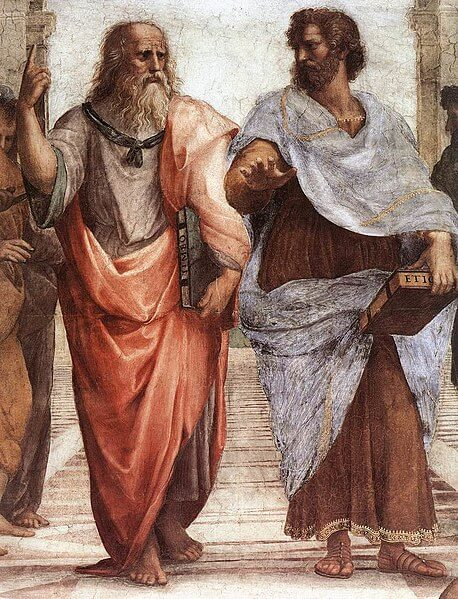
\includegraphics{assets/unit_3/U3_458px-Sanzio_01_Plato_Aristotle.jpg}

\emph{Graphic art of Plato and Aristotle.Photo Credit: \href{https://en.wikipedia.org/wiki/Aristotle\#/media/File:Sanzio_01_Plato_Aristotle.jpg}{Wikipedia}}

\hypertarget{overview-2}{%
\section*{Overview}\label{overview-2}}
\addcontentsline{toc}{section}{Overview}

Welcome to Unit 3!

Suppose you learn that a colleague at work is overcharging for certain items and pocketing the difference? You, being an honest and loyal employee, immediately take him aside and urge him to stop, reminding him that his actions are not only harmful to the company and against policy, but they are simply immoral. To your surprise, your colleague retorts, ``What I'm doing is harmless. The company is big enough that no one will even notice. I agree it's immoral but why should I care about being moral?'' How would you respond to this pointed question?

Have you ever wondered why you or anyone else should care about what is morally good or bad? Is it because you might get caught if you acted immorally, or because others would think less of you? What if you knew you would never get caught? Suppose no one, including God, would ever know if you acted unethically in a certain situation and, thus, no one would ever think less of you or treat you differently. Would you still choose the ethically good action? If so, why?

When we think about ethics, we are usually thinking of how to figure out ethical behaviour. But a deeper question, one that lies behind that question, is why anyone should be moral in the first place.

It is a question we cannot avoid forever because without an answer to it, the entire ethical enterprise is left hanging in the balance. Why put all this effort into trying to figure out what good ethical conduct is if there is no reason to pursue it in the first place? We must come up with some answer but how?

Furthermore, any discussion of the basis of our obligations toward other people immediately presents us with some deeper questions concerning our humanness. These include the following:
- What does it mean to be human?
- More importantly, what does it mean to be a person?
- Are all humans persons by virtue of their humanness?
- Alternatively, do persons have certain characteristics such as self-awareness, the ability to reason, or to carry out self-motivated activity, which certain humans have but others do not at certain stages of development?
- If so, at what point do we become persons with all the rights of personhood? Is it at the point of conception, at birth, or at some point either between these two, or even after the point of birth?

The way we answer these questions will affect our views on such key ethical issues as \textbf{abortion, infanticide, euthanasia, physician-assisted suicide, contraception, in vitro fertilization}, etc. For example, if humans are persons with all the moral rights thereof from conception on, then abortion at any stage of development will be as immoral as ending the life of a three year old child. On the other hand, if humans do not have the rights of personhood until the point of birth, or until some other definite point of development, then abortion, even infanticide, may be morally permissible until they reach that point. Similar reasoning could be applied to the other issues mentioned here.

Rather than focus on these individual issues, in this unit we'll try to
get behind them and explore the basis of our moral obligation. One thing to
remember is that when it comes to answering the question, `Why be moral?' one
answer we cannot give is, ``because it's the right thing to do,'' since, when we
ask, why be moral, we are asking precisely why we should care about doing the
right thing. How, then, can we answer it?

This question has been the subject of intense debate for thousands of years. In this unit, we'll take a short journey down a fascinating trail of case studies, secondary questions, new terms, and different answers to the main question which have been tried out. We'll come across terms like \textbf{Social Contract morality, psychological egoism} and \textbf{ethical egoism}. It is important to understand the meanings of these terms and the different perspectives they bring to our question, ``Why be moral?'' We'll even see if evolutionary biology can help us answer this foundational question about morality. Get ready to read about \textbf{the selfish gene} and \textbf{kin altruism}.

Last, we'll be introduced to the famous story of the Ring of Gyges, told by the ancient Greek philosopher, Plato. It's one of the most intriguing stories of all time relating to the question, why be moral, and it focuses our thoughts on this question. We'll take some time on it in the learning activities for this unit. Once you've read it, it will set the stage for the different answers we'll see to the question.

Let's plunge in. Why be moral?

\hypertarget{topics-2}{%
\section*{Topics}\label{topics-2}}
\addcontentsline{toc}{section}{Topics}

This unit is divided into 2 topics:

\begin{enumerate}
\def\labelenumi{\arabic{enumi}.}
\tightlist
\item
  Egoism \& Self-interest Morality\\
\item
  Social Contract Morality
\end{enumerate}

\hypertarget{learning-outcomes-2}{%
\subsection*{Learning Outcomes}\label{learning-outcomes-2}}
\addcontentsline{toc}{subsection}{Learning Outcomes}

When you have completed this unit, you should be able to:

\begin{itemize}
\tightlist
\item
  Explain key ethical concepts such as ethical egoism, psychological egoism, self-interest morality, and kin altruism.\\
\item
  Discuss knowledgeably Plato's famous story of the Ring of Gyges.\\
\item
  Discuss whether people would do what is right, even if no one would find out.
\end{itemize}

\hypertarget{activity-checklist-2}{%
\subsection*{Activity Checklist}\label{activity-checklist-2}}
\addcontentsline{toc}{subsection}{Activity Checklist}

Here is a checklist of learning activities you will benefit from in completing
this unit. You may find it useful for planning your work.

\begin{reflect}
\hypertarget{read-view-and-reflect-6}{%
\subsubsection*{Read, View and Reflect}\label{read-view-and-reflect-6}}
\addcontentsline{toc}{subsubsection}{Read, View and Reflect}

Read Chapter 6 on Egoism of your \emph{Introduction} textbook, Wolff, Jonathan. ~\emph{An Introduction to Moral Philosophy}. Watch the video related to the topic.

\hypertarget{wallet-case-study}{%
\subsubsection*{Wallet Case Study}\label{wallet-case-study}}
\addcontentsline{toc}{subsubsection}{Wallet Case Study}

Read and analyze the case study presented.

\hypertarget{read-view-and-reflect-7}{%
\subsubsection*{Read, View and Reflect}\label{read-view-and-reflect-7}}
\addcontentsline{toc}{subsubsection}{Read, View and Reflect}

Read Chapter 7: The Social Contract, in your \emph{Introduction} textbook\emph{.} Watch the videos related to the topic.

\hypertarget{key-terms-quiz-1}{%
\subsubsection*{Key Terms Quiz}\label{key-terms-quiz-1}}
\addcontentsline{toc}{subsubsection}{Key Terms Quiz}

Take the ungraded quiz to review important concepts.

\hypertarget{ethics-committee-response-ungraded}{%
\subsubsection*{Ethics Committee Response (ungraded)}\label{ethics-committee-response-ungraded}}
\addcontentsline{toc}{subsubsection}{Ethics Committee Response (ungraded)}

Meet with your Ethics Committee to discuss the case presented.

\hypertarget{assignment-2}{%
\subsubsection*{\texorpdfstring{\textbf{Assignment}}{Assignment}}\label{assignment-2}}
\addcontentsline{toc}{subsubsection}{\textbf{Assignment}}

Partner Project Presentation (30\%):
This assignment will be presented during weeks 5-10. You must choose a partner and topic this week (see Units 5-10 topics).
\end{reflect}

\hypertarget{resources-2}{%
\subsection*{Resources}\label{resources-2}}
\addcontentsline{toc}{subsection}{Resources}

Here are the resources you will need to complete this unit.
- Wolff, Jonathan. ~\emph{An Introduction to Moral Philosophy}. ~New York: W. W.
Norton \& Company, 2018. ~
- Other online resources will be provided in the unit.

\hypertarget{egoism}{%
\subsection*{Egoism}\label{egoism}}
\addcontentsline{toc}{subsection}{Egoism}

The first topic related to the question, why be moral, comes under the heading of Egoism. There are two kinds of egoism which we will examine, \textbf{psychological egoism} and \textbf{ethical egoism,} and the discussion of these concepts may surprise you. The theories developed around them are similar in certain respects yet give significantly different answers to the question, why be moral.

\textbf{Psychological egoism}, as its name suggests, is a psychological theory about human behaviour and claims that we, humans, cannot help but pursue that which is in our own best interest. It's not difficult to see what this means for our question, why be moral. If this theory is correct, it would make it virtually impossible for anyone to act morally \emph{unless she believed it was in her own best interest to do so}. It will be important to reflect on this theory in the reading to see if it merits our acceptance.

\textbf{Ethical egoism}, as its name indicates, is an ethical theory which teaches
that we have a right, and possibly even a duty, to pursue our own
self-interests. Following our self-interests is the morally right thing to do.

Our text book identifies two distinct forms of ethical egoism. According to one
form, acting in our own self-interest is the best way of advancing the good of
others around us because it is in our self-interest to do good for others. A
society works better when we all look out for the good of others; thus it is in
our best interest to act this way and promote this kind of society.

A different form of ethical egoism, however, holds that it is morally right to act in our own best interests, \emph{regardless of the consequences of others}. The best known proponent of this kind of pure ethical egoism is the Russian-American philosopher and novelist, Ayn Rand, who referred to the ``duty of selfishness.'' We will read briefly about her views in the text reading for this topic.

As we read the chapter on egoism in the Wolff text, think carefully about the
implications this theory, if true, would have for our question, why be moral.

\hypertarget{learning-activities-6}{%
\subsection*{Learning Activities}\label{learning-activities-6}}
\addcontentsline{toc}{subsection}{Learning Activities}

\begin{reflect}
\hypertarget{read-view-and-reflect-8}{%
\subsubsection*{Read, View and Reflect}\label{read-view-and-reflect-8}}
\addcontentsline{toc}{subsubsection}{Read, View and Reflect}

In the first activity, you are asked to read chapters 6 on Egoism of your
textbook, \emph{An Introduction to Moral Philosophy} by Jonathan Wolff. As you read,
be sure to take notes in your Learning Journal, defining key terms and
explaining key concepts. Study the chapter review summary, questions and key
terms. This will help you as you complete the assessments in this course.
Watch the following video that illustrates various types of egoism:

\hypertarget{wallet-case-study-1}{%
\subsubsection*{Wallet Case Study}\label{wallet-case-study-1}}
\addcontentsline{toc}{subsubsection}{Wallet Case Study}

\textbf{Introduction}

Read the following case study and answer the questions in your learning journal.
You are out for a walk in the park when you suddenly spot a wallet lying in the grass. ~Someone has lost it. Upon opening it, you find the I.D. of the owner and contact information; it is someone of whom you have never heard. ~You also find a substantial amount of cash. You have a number of options: leave the wallet alone and continue walking, mail it back to the owner with all its contents inside, or pocket the cash and either mail the wallet back or leave it on the grass. ~If you take the cash, no one will ever know. You think back to your ethics course and realize there are a number of perspectives on your situation.
For this case study, how would a psychological egoist, an ethical egoist, and an advocate of self-interest morality answer the following question: should you pocket the cash? ~Explain why they would each answer as they do.
\end{reflect}

\hypertarget{social-contract-morality}{%
\subsection*{Social Contract Morality}\label{social-contract-morality}}
\addcontentsline{toc}{subsection}{Social Contract Morality}

The second topic related to our question, why be moral, could hardly be more
different from the first. It comes under the heading, Social Contract Morality,
and suggests that moral rules in any society are the result of a social
contract, usually implicit, made between all members of the society. We realize,
say advocates of this theory, that it is in everyone's interests to develop
ethical rules which are to the benefit of all people, and teach them throughout
society. No society could function if everyone did as they wished. Might would
make right, thugs would rule, and life for those who survived would be filled
with fear and exhaustion.

We've seen the difference between the social contract theory and the previous
egoistic ones but can you also see a fundamental similarity between them? This
theory also teaches that the reason we should be moral is that it is in our best
interest to do so. As you read the section in the course text on The Social
Contract, reflect further on this similarity and also on whether it provides an
adequate basis for us to be moral. What problems or questions does it raise?

\hypertarget{learning-activities-7}{%
\subsection*{Learning Activities}\label{learning-activities-7}}
\addcontentsline{toc}{subsection}{Learning Activities}

\begin{reflect}
\hypertarget{read-view-and-reflect-9}{%
\subsubsection*{Read, View and Reflect}\label{read-view-and-reflect-9}}
\addcontentsline{toc}{subsubsection}{Read, View and Reflect}

In this activity, you are asked to read chapter 7, The Social Contract in your
textbook, \emph{An Introduction to Moral Philosophy,} by Jonathan Wolff. Take notes
on key terms and concepts.
Next, watch the following video to get a better understanding of social
contract morality.

\hypertarget{key-terms-quiz-ungraded-2}{%
\subsubsection*{Key Terms Quiz (ungraded)}\label{key-terms-quiz-ungraded-2}}
\addcontentsline{toc}{subsubsection}{Key Terms Quiz (ungraded)}

In order to review some of the major concepts from the text, take the following
unmarked quiz. Although you will not be evaluated on these terms, they will
assist you in the assignments for this course.
Match the following terms to their correct definition.
\end{reflect}

\hypertarget{assessment-2}{%
\subsection*{Assessment}\label{assessment-2}}
\addcontentsline{toc}{subsection}{Assessment}

\begin{assessment}
\hypertarget{assignment-ethics-committee-response-20-1}{%
\subsubsection*{Assignment: Ethics Committee Response (20\%)}\label{assignment-ethics-committee-response-20-1}}
\addcontentsline{toc}{subsubsection}{Assignment: Ethics Committee Response (20\%)}

After completing this unit, including the learning activities, you are asked to
analyze Plato's story of the Ring of Gyges from various perspectives. You will
work again with your Ethics Committee group to discuss the case and then post a
summary report online.

For this Ethics Committee meeting, analyze Plato's story of the Ring of Gyges (from the text reading, p.~88) and state how his key question, ``What would you do?'' might be answered by an ethical egoist, a psychological egoist, an advocate of self-interest morality, and a kin altruist. ~Then explain why you think each would answer as they do. (e.g.~\emph{If I was a \ldots.I would say\ldots{} ~Here is why.)}

As you meet with your Ethics Committee this week, discuss the story and take
notes. In your response, work with key terms and concepts from your readings.
(eg. \emph{If I was a \ldots.I would say\ldots about this case.})

Refer to the \textbf{grading criteria} in the Assessments section of this course.
Submit your report on Moodle by the end of the week.

\hypertarget{assignment-partner-project-presentation-30}{%
\subsubsection*{Assignment: Partner Project Presentation (30\%)}\label{assignment-partner-project-presentation-30}}
\addcontentsline{toc}{subsubsection}{Assignment: Partner Project Presentation (30\%)}

For this partner project, you will choose a specific ethical issue to address.
Please note that this is an argumentative project and not simply a discussion
project. Your presentation should be 12-15 minutes in length and have a visual
element (e.g.~PowerPoint). You will also have an additional 10 minutes at the
end of your presentation to answer questions and facilitate a class discussion.

Note that this assignment will be presented during weeks 5-10. You must choose a partner and topic this week (see Units 5-10 topics). Your Facilitator will hand out a sign-up sheet. Complete this before moving on to the next unit.

See more assignment details, including the \emph{grading criteria} in the Assessments section of this course.

\hypertarget{sign-up-for-the-partner-project-presentation}{%
\subsubsection*{Sign-up for the Partner Project Presentation}\label{sign-up-for-the-partner-project-presentation}}
\addcontentsline{toc}{subsubsection}{Sign-up for the Partner Project Presentation}

For this partner project, your group will choose a specific ethical issue to address.
Please note that this is an argumentative project and not simply a discussion
project. Your presentation should be 12-15 minutes in length and have a visual
element (e.g.~PowerPoint). You will also have an additional 10 minutes at the
end of your presentation to answer questions and facilitate a class discussion.
\end{assessment}

\begin{caution}
\textbf{Note} that this assignment will be presented during weeks 5-10. You must choose a group and topic this week (see Units 3-10 topics). Your Facilitator will hand out a sign-up sheet. Complete this before moving on to the next unit.
\end{caution}

See more assignment details, including the \emph{grading criteria} in the Assessments section of this course.

\hypertarget{checking-your-learning-2}{%
\section*{Checking your Learning}\label{checking-your-learning-2}}
\addcontentsline{toc}{section}{Checking your Learning}

\begin{progress}
Before you move on to the next unit, you may want to check to make sure that you are able to:

\begin{itemize}
\tightlist
\item
  Explain key ethical concepts such as ethical egoism, psychological egoism, self-interest morality, and kin altruism.\\
\item
  Discuss knowledgeably Plato's famous story of the Ring of Gyges.\\
\item
  Discuss whether people would do what is right, even if no one would find out.
\end{itemize}
\end{progress}

\hypertarget{how-to-determine-what-is-moral}{%
\chapter{How to Determine What is Moral}\label{how-to-determine-what-is-moral}}


\includegraphics{assets/unit_4/thinker-1294493_640.jpg}

\emph{Artistic sculpture. Photo Credit: \href{https://pixabay.com/en/thinker-at-a-loss-consider-play-1294493/}{Pixabay}}

\hypertarget{overview-3}{%
\section*{Overview}\label{overview-3}}
\addcontentsline{toc}{section}{Overview}

Have you ever had a disagreement with someone over what the correct ethical
action or point of view is in a certain situation? Perhaps, for example, a
person who has murdered three people and terrorized your community for the past
four months has just been arrested and found guilty with overwhelming evidence.
You say justice requires that this person be executed but your friend staunchly
disagrees. She argues that killing humans is wrong in all situations because
human life has intrinsic value and dignity regardless of what any person has
done.
Another example: you and a friend disagree about whether you should tell a lie to your employer in order to save a colleague's job who has been unfairly accused of padding her expense account. It's a complicated situation but by telling one small lie, you can lift the suspicion from your colleague. ``Of course you should lie!'' your friend confidently asserts. ``After all, it would be a gross injustice for her to be fired for something she didn't do, and what harm is there is telling the lie to prevent that injustice?'' You, however, are not so sure that lying is really that harmless.
Disagreements like this can arise over a host of morally perplexing dilemmas and when they do, we sometimes wonder how to resolve them.

This is the question we will be addressing in this unit, i.e., \textbf{how can we decide what good ethical behaviour is when we are faced with tough ethical choices?} Is there a procedure, or set of procedures, we can follow to help provide ethical guidance for the perplexing moral questions we all face from time to time? In other words, what does morality call us to do in these tough situations and how can we determine that?

There are three common theories of morality which set out answers to this question: \textbf{Justice as Fairness, Utilitarianism,} and \textbf{The Categorical Imperative}. In this unit we will read articles setting out each of these theories along with a basic rationale for each.

\hypertarget{topics-3}{%
\section*{Topics}\label{topics-3}}
\addcontentsline{toc}{section}{Topics}

This unit is divided into 3 topics:

\begin{enumerate}
\def\labelenumi{\arabic{enumi}.}
\tightlist
\item
  Understanding the Original Position\\
\item
  Utilitarianism\\
\item
  The Categorical Imperative
\end{enumerate}

\hypertarget{learning-outcomes-3}{%
\subsection*{Learning Outcomes}\label{learning-outcomes-3}}
\addcontentsline{toc}{subsection}{Learning Outcomes}

When you have completed this unit, you should be able to:

\begin{itemize}
\tightlist
\item
  Describe a number of foundational ethical ideas related to the question, ``Why be moral?'' such as the original position, utilitarianism, and the categorical imperative.\\
\item
  Suggest ways in which adhering to each of these concepts would influence the decision-making process when facing moral dilemmas.\\
\item
  Explain key objections to each of these concepts.
\end{itemize}

\hypertarget{activity-checklist-3}{%
\subsection*{Activity Checklist}\label{activity-checklist-3}}
\addcontentsline{toc}{subsection}{Activity Checklist}

Here is a checklist of learning activities you will benefit from in completing
this unit. You may find it useful for planning your work.

\begin{reflect}
\hypertarget{read-view-and-reflect-10}{%
\subsubsection*{Read, View and Reflect}\label{read-view-and-reflect-10}}
\addcontentsline{toc}{subsubsection}{Read, View and Reflect}

\begin{itemize}
\item
  Read pages 125-132 of your \emph{Readings} textbook. Watch the videos related to the topic.
\item
  Read pages 132-150 of your \emph{Readings} textbook. Watch the videos related to the topic.
\item
  Read pages 152-160 of your \emph{Readings} textbook. Watch the videos related to the topic.
\end{itemize}

\hypertarget{diamond-case-study}{%
\subsubsection*{Diamond Case Study}\label{diamond-case-study}}
\addcontentsline{toc}{subsubsection}{Diamond Case Study}

Read and analyze the case study presented.

\hypertarget{ethics-simulation-optional}{%
\subsubsection*{Ethics Simulation (Optional)}\label{ethics-simulation-optional}}
\addcontentsline{toc}{subsubsection}{Ethics Simulation (Optional)}

Explore the ethics simulation presented.

\hypertarget{key-terms-quiz-2}{%
\subsubsection*{Key Terms Quiz}\label{key-terms-quiz-2}}
\addcontentsline{toc}{subsubsection}{Key Terms Quiz}

Take the ungraded quiz to review important concepts.

\hypertarget{assignment-3}{%
\subsubsection*{\texorpdfstring{\textbf{Assignment}}{Assignment}}\label{assignment-3}}
\addcontentsline{toc}{subsubsection}{\textbf{Assignment}}

Ethics Committee Response (15\%)
\end{reflect}

\hypertarget{resources-3}{%
\subsection*{Resources}\label{resources-3}}
\addcontentsline{toc}{subsection}{Resources}

Here are the resources you will need to complete this unit.
- Wolff, Jonathan. ~\emph{Readings in Moral Philosophy}. ~New York: W. W. Norton \& Company, 2018.\\
- Other online resources will be provided in the unit.

\hypertarget{understanding-the-original-position}{%
\subsection*{Understanding the Original Position}\label{understanding-the-original-position}}
\addcontentsline{toc}{subsection}{Understanding the Original Position}

How can we decide what good ethical behaviour is when we are faced with tough
ethical choices? One answer, or theory of morality, called \textbf{`Justice as
Fairness'}, holds that the morally good, or just, course of action is the one
which is the fairest in the situation. How, though, do we figure out what is
fair, especially in a way that others will agree with us? How could anyone
figure out a thing like that?
Interestingly, John Rawls, a twentieth century American political philosopher, and an advocate of this view, has developed a well-known thought experiment to help us do precisely that. We will read about it in the article by him in our course readings for this unit. Be ready to figure out what he meant by such key terms as \textbf{the original position} and \textbf{veil of ignorance}. Without a clear grasp of these, we will not understand this thought experiment or Rawls' method.
We may need to read over certain parts a few times to really grasp these key concepts but, given the importance of preparing to face tough moral dilemmas, it will be worth the effort. We'll also have opportunities to discuss them with colleagues in this class to help gain a working knowledge of them. In the end, let's try to answer the question for ourselves: How can I determine what is moral?

\hypertarget{learning-activities-8}{%
\subsection*{Learning Activities}\label{learning-activities-8}}
\addcontentsline{toc}{subsection}{Learning Activities}

\begin{reflect}
\hypertarget{read-view-and-reflect-11}{%
\subsubsection*{Read, View and Reflect}\label{read-view-and-reflect-11}}
\addcontentsline{toc}{subsubsection}{Read, View and Reflect}

In the first activity, you are asked to read pages 125-132 of your textbook, \emph{Readings in Moral Philosophy} by Jonathan Wolff. As you read, be sure to take notes in your Learning Journal, defining key terms and explaining key concepts. Study the chapter review summary, questions and key terms. This will help you as you complete the assessments in this course.

Next, choose from the following videos to learn more about the key terms from this section.
\end{reflect}

\hypertarget{topic-2-utilitarianism}{%
\section*{Topic 2: Utilitarianism}\label{topic-2-utilitarianism}}
\addcontentsline{toc}{section}{Topic 2: Utilitarianism}

\textbf{Introduction}
Another answer to the question of how to determine what is moral is called \textbf{utilitarianism}. This view teaches that morally good actions are those that, on balance, bring about the greatest good or happiness in any given situation. This theory seems rather intuitive to many people and, not surprisingly, has been around for a long time. Nineteenth century British philosopher, John Stuart Mill, its best known representative, has written the article we'll read to see how he develops it.
As you're reading his article, ask yourself if you can think of any problems with it. Serious objections have been raised against this view which is why many people have preferred the next answer we will consider.

\hypertarget{learning-activities-9}{%
\subsection*{Learning Activities}\label{learning-activities-9}}
\addcontentsline{toc}{subsection}{Learning Activities}

\begin{reflect}
\hypertarget{read-view-and-reflect-12}{%
\subsubsection*{Read, View and Reflect}\label{read-view-and-reflect-12}}
\addcontentsline{toc}{subsubsection}{Read, View and Reflect}

Read pages 132-150 of your textbook, \emph{Readings in Moral Philosophy} by Jonathan
Wolff. Take notes on key terms and concepts.
Next, choose from the following videos to get a better understanding of
utilitarianism.
\end{reflect}

\hypertarget{the-categorical-imperative}{%
\subsection*{The Categorical Imperative}\label{the-categorical-imperative}}
\addcontentsline{toc}{subsection}{The Categorical Imperative}

Our third answer to the question of how to determine what is morally good action was set out by the eighteenth-century German philosopher, Immanuel Kant. He rejected utilitarianism and took an entirely different approach. His theory is that the morality of any action does not depend on its consequences or effects because those same effects, namely happiness and pleasure, could be produced by a whole variety of actions, many of which would not be just. In other words, happiness and pleasure are unreliable guides to determining morally just actions.
Rather, he said, the morality of an action depends upon whether it fulfills our duty to follow ethical rules. What rules? Kant said we can develop rules which are drawn from one supreme principle of morality which he called \textbf{The Categorical Imperative}. His moral system is often called duty-based, or rule-based ethics, as opposed to the consequence-based ethics of utilitarianism. As we read the article by this philosopher, let's see what we think about this way of determining morally just action.

\hypertarget{learning-activities-10}{%
\subsection*{Learning Activities}\label{learning-activities-10}}
\addcontentsline{toc}{subsection}{Learning Activities}

\begin{reflect}
\hypertarget{read-view-and-reflect-13}{%
\subsubsection{Read, View and Reflect}\label{read-view-and-reflect-13}}

Read pages 152-160 of your textbook, \emph{Readings in Moral Philosophy} by Jonathan
Wolff. Take notes on key terms and concepts.
Next, choose from the following videos to get a better understanding of
utilitarianism.

\hypertarget{diamond-case-study-1}{%
\subsubsection*{Diamond Case Study}\label{diamond-case-study-1}}
\addcontentsline{toc}{subsubsection}{Diamond Case Study}

Read the following case study and consider what you would do in the situation.
What ethical issues arise?
You, a follower of utilitarian ethics and a poor college student, are enjoying an evening visiting with two friends. ~One is a parent of seven children with limited financial means who holds to Immanuel Kant's categorical imperative, while the other is a wealthy business owner who happens to be a follower of John Rawls' theory of justice built around the concept of the original position. ~Your topic of discussion is the relative merits of these three ethical concepts. Suddenly someone enters the room with a small box of valuable diamonds and says they have been donated to your group of three by a wealthy philanthropist who wishes to remain anonymous. The donor asked that they be divided ``justly'' among you but has left the definition of justice up to you. ~How would each of you say they should be divided? How does each ethical concept, the categorical imperative, the original position, and utilitarianism influence each answer?
\end{reflect}

\begin{caution}
\emph{Note that this is an ungraded activity, but you are encouraged to write your answers in your notes or reflective journal. You may be asked to review this case or similar cases in your class discussion groups. This practice of analyzing a case, contemplating various perspectives, and presenting an argument will help you in your assessments for this course.}
\end{caution}

\begin{reflect}
\hypertarget{ethics-simulation-optional-1}{%
\subsubsection*{Ethics Simulation (Optional)}\label{ethics-simulation-optional-1}}
\addcontentsline{toc}{subsubsection}{Ethics Simulation (Optional)}

Now that you have learned about the main ethical theories and principles, look
for opportunities to challenge yourself! Look up ethical case studies or
simulations online and see if you can provide sound reasoning and link to the
theories you have learned.
One app in particular you may want to try is Ethical Decision Making (below). It helps you go through the options to make tough ethical decisions.

//todo \#2
Ethical Decision Making - Apps on Google Play

Feel free to share any resources you find with your classmates!

\hypertarget{key-terms-quiz-ungraded-3}{%
\subsubsection*{Key Terms Quiz (ungraded)}\label{key-terms-quiz-ungraded-3}}
\addcontentsline{toc}{subsubsection}{Key Terms Quiz (ungraded)}

In order to review some of the major concepts from the text, take the following
unmarked quiz. Although you will not be evaluated on these terms, they will
assist you in the assignments for this course.
Match the following terms to their correct definition.
\end{reflect}

\hypertarget{assessment-3}{%
\subsection*{Assessment}\label{assessment-3}}
\addcontentsline{toc}{subsection}{Assessment}

\begin{assessment}
\hypertarget{assignment-ethics-committee-response-20-2}{%
\subsubsection*{Assignment: Ethics Committee Response (20\%)}\label{assignment-ethics-committee-response-20-2}}
\addcontentsline{toc}{subsubsection}{Assignment: Ethics Committee Response (20\%)}

After completing this unit, including the learning activities, you are asked to
meet with your Ethics Committee and discuss the following:

For the following ethical theories, Justice as fairness, the categorical imperative, and utilitarianism, explain the answer you think an advocate of each position would give to the following question:

\emph{Should the government provide housing and a food allowance for homeless people?}

As you meet with your Ethics Committee this week, discuss the question and provide some of the key reasoning you think each perspective would use in coming to what they believe to be a just solution. In other words, the utilitarian would point out. . . and say. . ., etc.

In your response, work with key terms and concepts from your readings. (eg. \emph{If I was a \ldots.I would say\ldots about this case.})

Submit your report on Moodle by the end of the week.

\hypertarget{assignment-reflective-journal-ungraded-practice-1}{%
\subsubsection*{Assignment: Reflective Journal (ungraded practice)}\label{assignment-reflective-journal-ungraded-practice-1}}
\addcontentsline{toc}{subsubsection}{Assignment: Reflective Journal (ungraded practice)}

For your second Reflective Journal in this course, you are invited to write about what you have learned in this unit. Remember that you should consider your journal as a place for you to try out new ideas, to test your assumptions, and to possibly share what you are learning with your community.
After completing this unit, including the learning activities, you are asked to write a 250-400 word journal entry responding to the following question: ``Why Be Moral?''

\hypertarget{discussion-responses-1}{%
\subsubsection*{Discussion Responses}\label{discussion-responses-1}}
\addcontentsline{toc}{subsubsection}{Discussion Responses}

After you have finished your journal assignment, you will share your responses in class with your peers. You will then be asked to add 1-2 more ideas to your journal response, highlighting what you learned from the discussion with your peers.
\end{assessment}

\hypertarget{checking-your-learning-3}{%
\section*{Checking your Learning}\label{checking-your-learning-3}}
\addcontentsline{toc}{section}{Checking your Learning}

\begin{progress}
Before you move on to the next unit, you may want to check to make sure that you are able to:

\begin{itemize}
\tightlist
\item
  Describe a number of foundational ethical ideas related to the question,
  ``Why be moral?'' such as the original position, utilitarianism, and the
  categorical imperative.\\
\item
  Suggest ways in which adhering to each of these concepts would influence the decision-making process when facing moral dilemmas.\\
\item
  Explain key objections to each of these concepts.
\end{itemize}
\end{progress}

\hypertarget{free-speech-and-its-limits}{%
\chapter{Free Speech and its Limits}\label{free-speech-and-its-limits}}


\includegraphics{assets/unit_5/U5_117704119_65c60568e1_b.jpg}

\emph{Man with a poster of free speech. Photo Credit: \href{https://flickr.com/photos/sjgibbs/117704119}{flickr photo by sjgibbs80}}

\hypertarget{overview-4}{%
\section*{Overview}\label{overview-4}}
\addcontentsline{toc}{section}{Overview}

Welcome to Unit 5. In this unit we are turning our attention to the ethics of free speech and expression. You have probably noticed how deeply people value and appreciate the right to free speech. Many, in fact, would believe they, and their society, had lost something profoundly important if they ever lost this right.
In many countries, the right to free speech is seen as one of the foundations of society, as virtually an unquestioned cultural assumption. Those who dare to challenge, or even question, it do so at their peril. In other words, it is a foundational right upon which we base many other rights.
Perhaps you've wondered why this is so and how things got to be this way. How did the right to free speech gain such an elevated standing in people's minds? Moreover, should it ever be limited or is it simply an absolute principle with no exceptions? If it should be limited, when, and why? What could possibly be so important that it would call for a limitation on one's free speech?

Let's begin by exploring our own personal views on the matter. Suppose someone you know believes something with which you and many of your friends flatly \textbf{disagree}. Should they have the right to express this belief? Most of us would probably answer, yes, to this question.
What, however, if you and your companions don't simply \emph{disagree} with this viewpoint but actually find it \emph{disturbing}? Should the right to free speech and expression still hold?
Suppose it's worse than that. Suppose you, and plenty of people you know, actually find this viewpoint \emph{disgusting}? What then? Should the person still be given the right to express this view?
One last `what if' question: what if you believe the expression of this viewpoint would be genuinely \emph{dangerous} to some person or group of people in your society? Does the right to free speech guarantee their right to express the view even in this case?

The point of these `what if' scenarios is to test our views on this right and to raise a critical question for this unit: how far does the right to free speech go? We will see that this question cannot be answered without first establishing the basis for free speech in the first place.
Notice that our basis for free speech cannot simply be that the government decrees this right, since the very question at stake is what moral basis governments have doing so. Our readings for this unit will expose us both to a proposed \emph{moral foundation} for the right to free speech and a case for certain \emph{limitations} to be placed upon it. Once we understand the arguments made for both, we will be in a position to reflect on them and decide whether we would draw the lines in different places than these authors have.

\hypertarget{topics-4}{%
\section*{Topics}\label{topics-4}}
\addcontentsline{toc}{section}{Topics}

This unit is divided into two topics:

\begin{enumerate}
\def\labelenumi{\arabic{enumi}.}
\tightlist
\item
  A Moral Foundation for Free Speech\\
\item
  Pornography and Limits on Free Speech
\end{enumerate}

\hypertarget{learning-outcomes-4}{%
\subsection*{Learning Outcomes}\label{learning-outcomes-4}}
\addcontentsline{toc}{subsection}{Learning Outcomes}

When you have completed this unit, you should be able to:

\begin{itemize}
\tightlist
\item
  Explain John Stuart Mill's four grounds for the freedom of expression.\\
\item
  Describe limitations on freedom of expression suggested by John Stuart Mill and his rationale for such limits.\\
\item
  Discuss why some who still favour freedom of speech believe pornography should not be freely distributed.\\
\item
  Show how John Stuart Mill's Harm Principle is foundational to the question of when and why limits should be placed on free speech.
\end{itemize}

\hypertarget{activity-checklist-4}{%
\subsection*{Activity Checklist}\label{activity-checklist-4}}
\addcontentsline{toc}{subsection}{Activity Checklist}

Here is a checklist of learning activities you will benefit from in completing
this unit. You may find it useful for planning your work.

\begin{reflect}
\hypertarget{read-view-and-reflect-14}{%
\subsubsection*{Read, View and Reflect}\label{read-view-and-reflect-14}}
\addcontentsline{toc}{subsubsection}{Read, View and Reflect}

\begin{itemize}
\tightlist
\item
  Read John Stuart Mill's article on free speech and its limits in pages 252-268 of your \emph{Readings} textbook.\\
\item
  Read the article by Catherine Mackinnon on pornography, civil rights, and free speech, in pages 268-278 of your \emph{Readings} textbook.
\end{itemize}

\hypertarget{controversial-speaker-case-study}{%
\subsubsection*{Controversial Speaker Case Study}\label{controversial-speaker-case-study}}
\addcontentsline{toc}{subsubsection}{Controversial Speaker Case Study}

Read and analyze the case study presented.

\hypertarget{key-terms-quiz-3}{%
\subsubsection*{Key Terms Quiz}\label{key-terms-quiz-3}}
\addcontentsline{toc}{subsubsection}{Key Terms Quiz}

Take the ungraded quiz to review important concepts.

\hypertarget{ethics-committee-response-ungraded-1}{%
\subsubsection*{Ethics Committee Response (ungraded)}\label{ethics-committee-response-ungraded-1}}
\addcontentsline{toc}{subsubsection}{Ethics Committee Response (ungraded)}

Meet with your Ethics Committee to discuss the case presented.
\#\#\#\# \textbf{Assignment} \{-\}

Ethics Video (15\%): This week you will select a topic for your video. The video must be posted on Moodle by the end of week 9.
\end{reflect}

\hypertarget{resources-4}{%
\subsection*{Resources}\label{resources-4}}
\addcontentsline{toc}{subsection}{Resources}

Here are the resources you will need to complete this unit.

\begin{itemize}
\tightlist
\item
  Wolff, Jonathan. ~\emph{Readings in Moral Philosophy}. ~New York: W. W. Norton \& Company, 2018.\\
\item
  Other online resources will be provided in the unit.
\end{itemize}

\hypertarget{a-moral-foundation-for-free-speech}{%
\section*{A Moral Foundation for Free Speech}\label{a-moral-foundation-for-free-speech}}
\addcontentsline{toc}{section}{A Moral Foundation for Free Speech}

Is free speech merely a personal preference, something we happen to like or prefer? Or is something we have a genuine moral right to possess? If so, it will require a moral basis, a set of reasons for thinking our society \emph{ought} to have and protect this right.
Furthermore, if we don't know \emph{why} we ought to have this right, we also have no way of deciding if, when, or why it should ever be limited. Once its basis is known, we can then consider whether a certain practice or idea would constitute an exception to this basis or go beyond its mandate.
Our first reading by John Stuart Mill, a nineteenth-century British philosopher who is sometimes referred to as the apostle of liberty, sets out a classical foundation for the right to free speech. In this classical article, Mill argued that minority views in a society must be given the right to be expressed, whether people believe they are true or false, and that we are all worse off if they are restricted. It will be important for us to catch Mill's reasons for this position because they will be useful in answering the follow-up question, namely, should free speech ever be limited.

\hypertarget{learning-activities-11}{%
\subsection*{Learning Activities}\label{learning-activities-11}}
\addcontentsline{toc}{subsection}{Learning Activities}

\begin{reflect}
\hypertarget{read-view-and-reflect-15}{%
\subsubsection*{Read, View and Reflect}\label{read-view-and-reflect-15}}
\addcontentsline{toc}{subsubsection}{Read, View and Reflect}

In the first activity, you are asked to read John Stuart Mill's article on free speech and its limits in pages 252-268 of your textbook, \emph{Readings in Moral Philosophy} by Jonathan Wolff. As you read, take notes in your Learning Journal, defining key terms and explaining key concepts.
Next, choose from the following videos to learn more about key terms from this
topic.
\end{reflect}

\hypertarget{pornography-and-limits-on-free-speech}{%
\section*{Pornography and Limits on Free Speech}\label{pornography-and-limits-on-free-speech}}
\addcontentsline{toc}{section}{Pornography and Limits on Free Speech}

If we agree that the right to free speech has a sound moral basis, does this
mean it is an absolute right with no exceptions? Or could there be certain
limitations placed on it even while maintaining it as a genuine right? In other
words, how far does this right go? If certain limitations are legitimate, what
are they and what basis could be given for them?
\emph{Disagreement} appears to be a weak basis for limiting free speech. The fact that some people \emph{disagree} with something you or I believe hardly seems like a proper reason to limit our free expression of that belief. Virtually every view point has its detractors and if we followed this principle consistently, it would lead to the collapse of the right to free speech. If, however, \emph{disagreement} does not constitute a good reason for limiting free speech, then what does?
In our second reading, we turn to this question. Catherine MacKinnon, an American lawyer and activist, presents us with a case in which she believes free speech ought to be limited, namely, pornography. She will argue both that free speech is important but that it should be limited in this one case. It will be important for us to follow her argument for both claims and consider our own stance toward them.

\hypertarget{learning-activities-12}{%
\subsection*{Learning Activities}\label{learning-activities-12}}
\addcontentsline{toc}{subsection}{Learning Activities}

\begin{reflect}
\hypertarget{read-view-and-reflect-16}{%
\subsection*{Read, View and Reflect}\label{read-view-and-reflect-16}}
\addcontentsline{toc}{subsection}{Read, View and Reflect}

Read the article by Catherine Mackinnon on pornography, civil rights, and free
speech, in pages 268-278 of your textbook, \emph{Readings in Moral Philosophy,} by
Jonathan Wolff. As you read, take notes in your Learning Journal, defining key
terms and explaining key concepts.
Next, choose from the following videos to learn more about key terms from this
topic.

\hypertarget{controversial-speaker-case-study-1}{%
\subsubsection*{Controversial Speaker Case Study}\label{controversial-speaker-case-study-1}}
\addcontentsline{toc}{subsubsection}{Controversial Speaker Case Study}

Read and analyse the following case study.
A controversial person is coming to your community planning on giving a public lecture in the community hall.The event which has been widely publicized has drawn protests from those who are petitioning the organizers to cancel the event. ~They argue that this speaker's views are offensive and should be neither tolerated nor even publicly expressed. From the course readings, how do you think John Stuart Mill would respond if he were one of the organizers? ~Tell why you believe he would respond this way. Do you agree with him? Why or why not?
\end{reflect}

\begin{caution}
\textbf{Note} that you may be asked to review this case or similar cases in your class discussion groups. You may want to prepare by relating the case to your readings. Specifically, identify the ethical issues and terms to help explain the case.
\end{caution}

\begin{reflect}
\hypertarget{activity-key-terms-quiz-ungraded}{%
\subsubsection*{Activity : Key Terms Quiz (ungraded)}\label{activity-key-terms-quiz-ungraded}}
\addcontentsline{toc}{subsubsection}{Activity : Key Terms Quiz (ungraded)}

In order to review some of the major concepts from the text, take the following
unmarked quiz. Although you will not be evaluated on these terms, they will
assist you in the assignments for this course.
Match the following terms to their correct definition.
\end{reflect}

\hypertarget{assessment-4}{%
\subsection*{Assessment}\label{assessment-4}}
\addcontentsline{toc}{subsection}{Assessment}

\begin{assessment}
\hypertarget{assignment-ethics-committee-response-10}{%
\subsubsection*{Assignment: Ethics Committee Response (10\%)}\label{assignment-ethics-committee-response-10}}
\addcontentsline{toc}{subsubsection}{Assignment: Ethics Committee Response (10\%)}

After completing this unit, including the learning activities, you are asked to
meet with your Ethics Committee and complete the following:

Produce a one-page report stating, first, what you believe to be the moral
\textbf{basis/foundation} for freedom of speech, and, second, any \textbf{examples} where
free speech should be limited. ~Thirdly, provide your \textbf{rationale} for each
example of a limitation and show how it still fits with your stated foundation
for free speech.

As you collaborate on this assignment, be sure to refer to the \textbf{grading
criteria} in the Assessments section of this course. Submit your report on
Moodle by the end of the week.

\hypertarget{ethics-video-assignment-choose-your-topic-15}{%
\subsubsection*{Ethics Video Assignment: Choose Your Topic (15\%)}\label{ethics-video-assignment-choose-your-topic-15}}
\addcontentsline{toc}{subsubsection}{Ethics Video Assignment: Choose Your Topic (15\%)}

For this assignment, you'll be asked to create a 2 minute video articulating a
moral viewpoint on one of the following issues: free speech, sexual morality,
abortion, euthanasia, or torture. Then, drawing upon the
readings, make a concise case for this viewpoint.

Your video must include the following elements:

\begin{itemize}
\tightlist
\item
  A clear statement of the ethical issue being addressed:
  what is the ethical question at hand?
\item
  Your proposed answer to this question.\\
\item
  At least one reason for your answer.\\
\item
  A professional and well-prepared appearance to the video as a whole:
  this may require rehearsing it once or twice. This video must be posted on Moodle by the end of week 9. ~If you choose to post it online outside of Moodle (e.g.~YouTube), please provide the URL.
\end{itemize}
\end{assessment}

\begin{caution}
\textbf{You will write 3 posts (150 words each) responding to three videos presented by your classmates, stating your agreement or disagreement with the arguments in the video, and explaining why you agree or disagree.}
\end{caution}

\hypertarget{checking-your-learning-4}{%
\section*{Checking your Learning}\label{checking-your-learning-4}}
\addcontentsline{toc}{section}{Checking your Learning}

\begin{progress}
Before you move on to the next unit, you may want to check to make sure that you are able to:

\begin{itemize}
\tightlist
\item
  Explain John Stuart Mill's four grounds for the freedom of expression.\\
\item
  Describe limitations on freedom of expression suggested by John Stuart Mill and his rationale for such limits.\\
\item
  Discuss why some who still favour freedom of speech believe pornography should not be freely distributed.\\
\item
  Show how John Stuart Mill's Harm Principle is foundational to the question of when and why limits should be placed on free speech.
\end{itemize}
\end{progress}

\hypertarget{sexual-morality}{%
\chapter{Sexual Morality}\label{sexual-morality}}

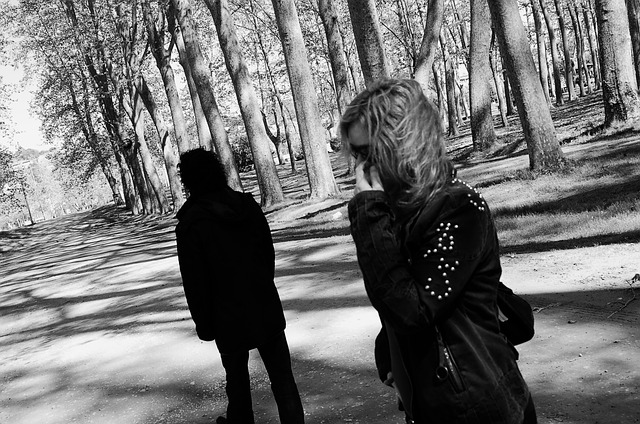
\includegraphics{assets/unit_6/portrait-119851_640.jpg}

\emph{image of two people standing across each other in the woods. Photo Credit: \href{https://pixabay.com/en/portrait-anger-people-couple-119851/}{Pixabay}}

\hypertarget{overview-5}{%
\section*{Overview}\label{overview-5}}
\addcontentsline{toc}{section}{Overview}

Welcome to unit six. In this unit we will be addressing the sensitive topic of
date rape and the influence of alcohol. It's a topic we need to treat with care
and understanding. Defining key terms and concepts will be especially important
here.
Most of us have some idea of what is meant by the term \textbf{date rape} and we know it is like other cases of rape in some ways but unlike them in others. What exactly are the differences and why do they matter?

In one of our readings we will see date rape defined as a sexual act which falls into the gray area between \textbf{consensual sex} and \textbf{aggressive rape}. If this definition is correct, then it leads us to one of the most important concepts in this discussion, namely, the concept of \textbf{consent}, which normally represents the dividing line between consensual sex and rape in general.
While obtaining consent is normally considered unproblematic, this is not always the case in date rape and it has led to a distinction between \textbf{valid consent} and \textbf{silent submission}. Understanding the difference between these two ideas is critical because it can constitute the difference between an act of date rape and one of consensual sex.

In one of our readings for this unit, Nicholas Dixon, an American professor of philosophy, introduces the role of alcohol into this discussion and argues that it is a critical factor precisely because it complicates the process of determining consent.
In another article we will read, Conor Kelly, an American professor and researcher in theological ethics, raises the concept of \textbf{hookup culture}. This refers to the increasingly common practice of engaging in sexual activity with no expectation of a longer-term commitment. She presents us with a foundational ethical question, especially from a feminist ethical point of view: Does the rise and wide acceptance of hookup culture represent an abuse of women or is it an expression of female liberation?

Here are some vital starting questions raised in our first reading by Lois Pineau, an American philosopher, for us to consider as we think about these issues: If a man gets a woman drunk and then has sex with her, would it count as rape? It would seem so but, then, what precisely constitutes the act of ``getting her drunk?'' What if she was happy to go along with the drinking? Where is the line to be drawn? The situation is further complicated, adds Pineau, if a woman has engaged in provocative behaviour earlier.
Pineau suggests that one way to approach this issue is to shift focus from questions like these and ask what is required for sexual activity to go well. What conditions must be met for this to occur? She suggests one condition for sexual activity going well by introducing the concept of \textbf{communicative sexuality.} It will be important for us both to understand and reflect on this concept.
Sometimes a woman simply goes along, says Pineau, either because her resistance is broken down, perhaps by alcohol or peer pressure, or because she fears a worse outcome if she resists. In other words, she says, sometimes \textbf{assault} is mistaken for \textbf{seduction}, which implies \textbf{consent}. In the end, Pineau argues that these serious problems can be dealt with by practicing communicative sexuality.
In our learning activities, we'll have an opportunity to interact with classmates and help each other fine-tune our understanding of these important concepts. Well also reflect on our own ethical stance on the key questions involved in this sensitive topic.

\hypertarget{topics-5}{%
\subsection*{Topics}\label{topics-5}}
\addcontentsline{toc}{subsection}{Topics}

This unit is divided into two topics:

\begin{enumerate}
\def\labelenumi{\arabic{enumi}.}
\tightlist
\item
  Date Rape\\
\item
  Alcohol \& Rape\\
\item
  Hookup Culture \& Women's Liberation
\end{enumerate}

\hypertarget{learning-outcomes-5}{%
\subsection*{Learning Outcomes}\label{learning-outcomes-5}}
\addcontentsline{toc}{subsection}{Learning Outcomes}

When you have completed this unit you should be able to:

\begin{itemize}
\tightlist
\item
  Describe how cultural assumptions sometimes lead to situations involving moral dilemmas of a sexual nature.\\
\item
  Discuss the importance of consent in determining the morality of a sexual encounter.\\
\item
  State the moral complexities surrounding impaired sexual activity
\item
  Explain how both date rape and alcohol use sometimes create gray areas between fully consensual sex and aggressive rape.\\
\item
  Define the term, hookup culture, and discuss the question this raises regarding the advancement of women's rights.\\
\item
  Discuss intelligently a number of rape myths.
\end{itemize}

\hypertarget{activity-checklist-5}{%
\subsection*{Activity Checklist}\label{activity-checklist-5}}
\addcontentsline{toc}{subsection}{Activity Checklist}

Here is a checklist of learning activities you will benefit from in completing this unit. You may find it useful for planning your work.

\begin{reflect}
\hypertarget{read-view-and-reflect-17}{%
\subsubsection*{Read, View and Reflect}\label{read-view-and-reflect-17}}
\addcontentsline{toc}{subsubsection}{Read, View and Reflect}

\begin{itemize}
\item
  Read the section on sexual morality by Lois Pineau (pages 293-306) of your \emph{Readings} textbook. Watch the videos related to the topic.
\item
  Read the section on sexual morality by Nicholas Dixon (pages 306-316) of your \emph{Readings} textbook. Watch the videos related to the topic.
\item
  Read the section on hookup culture, (pages 316-328) of your \emph{Readings} textbook.
\end{itemize}

\hypertarget{stuck-in-the-middle-case-study}{%
\subsubsection*{Stuck in the Middle Case Study}\label{stuck-in-the-middle-case-study}}
\addcontentsline{toc}{subsubsection}{Stuck in the Middle Case Study}

Read and analyze the case study presented.

\hypertarget{key-terms-quiz-4}{%
\subsubsection*{Key Terms Quiz}\label{key-terms-quiz-4}}
\addcontentsline{toc}{subsubsection}{Key Terms Quiz}

Take the ungraded quiz to review important concepts.

\hypertarget{resources-5}{%
\subsection*{Resources}\label{resources-5}}
\addcontentsline{toc}{subsection}{Resources}

Here are the resources you will need to complete this unit.
- Wolff, Jonathan. ~\emph{Readings in Moral Philosophy}. ~New York: W. W. Norton \& Company, 2018.\\
- Other online resources will be provided in the unit
\end{reflect}

\hypertarget{date-rape}{%
\section*{Date Rape}\label{date-rape}}
\addcontentsline{toc}{section}{Date Rape}

One of the first questions we need to ask is what, exactly, constitutes \textbf{date rape} and how it is different from rape in general? When can a person justifiably claim to have been ``date-raped?'' In our first reading, Lois Pineau, an American philosopher, writes that date rape falls into a gray area between \textbf{consensual sex} and \textbf{aggressive rape}.
If she is correct, then we come directly to one of the most important concepts in this discussion, namely, \textbf{consent}, which represents the dividing line between consensual sex and rape in general. In most situations, we are well aware of how to give consent and normally think we know when we have given or withheld it. When someone invites us to be involved in their work project, for instance, we either agree to get involved or we do not. The notion of consent seems unproblematic. In the issue of date rape, however, complexities can arise in determining when genuine consent has been given.

\hypertarget{learning-activities-13}{%
\subsection*{Learning Activities}\label{learning-activities-13}}
\addcontentsline{toc}{subsection}{Learning Activities}

\begin{reflect}
\hypertarget{read-view-and-reflect-18}{%
\subsubsection*{Read, View and Reflect}\label{read-view-and-reflect-18}}
\addcontentsline{toc}{subsubsection}{Read, View and Reflect}

In the first activity, you are asked to read the section on date rape by Lois
Pineau (pages 293-306) of your textbook, \emph{Readings in Moral Philosophy} by
Jonathan Wolff. As you read, take notes in your Learning Journal, defining key
terms and explaining key concepts.
Next, watch the following videos to learn more about key terms from this topic.

Also, see the following resource on sexual assault:
\url{http://sacha.ca/resources/statistics}
\end{reflect}

\hypertarget{alcohol-rape}{%
\section*{Alcohol \& Rape}\label{alcohol-rape}}
\addcontentsline{toc}{section}{Alcohol \& Rape}

As we noted earlier, in the issue of date rape, complicating factors can arise in determining when genuine consent has been given and one of the most common ones is presented by the role of alcohol. Nicholas Dixon, an American philosopher, raises this factor and it leads him to speak of \textbf{impaired sex}. The discussion over alcohol is especially important since it can add confusion precisely at the point of consent which represents the dividing line between legitimate sexual activity and rape. As Pineau points out, a person's consumption of alcohol can affect their ability to give consent.
If a woman is so incapacitated by alcohol that she cannot meaningfully give consent, then would a sexual act constitute rape? Does anything change if she said ``yes'' while in this condition, or had engaged in provocative behaviour earlier?
On the other hand, suppose a woman's inhibitions have been reduced by alcohol and she gives her consent but later regrets it, claiming it was out of sync with her long-held values? Does a sexual act in this case count as rape? Why or why not?
This has led to the distinction noted earlier between \textbf{valid consent} and \textbf{silent submission}.

\hypertarget{learning-activities-14}{%
\subsection*{Learning Activities}\label{learning-activities-14}}
\addcontentsline{toc}{subsection}{Learning Activities}

\begin{reflect}
\hypertarget{read-view-and-reflect-19}{%
\subsubsection*{Read, View and Reflect}\label{read-view-and-reflect-19}}
\addcontentsline{toc}{subsubsection}{Read, View and Reflect}

Read the section on alcohol and rape by Nicholas Dixon (pages 306-316) of your textbook, \emph{Readings in Moral Philosophy} by Jonathan Wolff. Take notes defining key terms and ideas. Study the chapter review summary, questions and key terms.
Next, watch the following videos to learn more about key terms from this topic.
\end{reflect}

\hypertarget{hookup-culture}{%
\section*{Hookup Culture}\label{hookup-culture}}
\addcontentsline{toc}{section}{Hookup Culture}

Date rape does not happen in isolation. It occurs within a social context, and a key feature of the current social context is described by the term, \textbf{hookup culture.} This term is introduced to us by Conor Kelly in the article we will read by her for this topic. It refers to the practice of engaging in sexual activity with no expectation by either party of a longer-term relationship.
As Kelly points out, hookup culture is increasingly accepted in our world. What we may not have noticed, however, is that it raises a key ethical question, one that she puts to us from the perspective of feminist ethics: \textbf{Does hookup culture represent a step forward for women's rights or is it, by nature, sexist and anti-women?} Is it an expression of increased freedom and equality, or does it, in effect, treat women as simply means used by men to have more free sex with no strings attached?
As we read Kelly's article, let's understand the concept of hookup culture and wrestle with this question. We'll have an opportunity to see what this cultural practice means for the task of determining helpful guiding principles to apply to the maze of questions surrounding date rape.

\hypertarget{learning-activities-15}{%
\subsection*{Learning Activities}\label{learning-activities-15}}
\addcontentsline{toc}{subsection}{Learning Activities}

\begin{reflect}
\hypertarget{read-and-reflect}{%
\subsubsection*{Read and Reflect}\label{read-and-reflect}}
\addcontentsline{toc}{subsubsection}{Read and Reflect}

Read the section on hookup culture, (pages 316-328) of your textbook, \emph{Readings in Moral Philosophy} by Jonathan Wolff. Take notes defining key terms and ideas.
Study the chapter review summary, questions and key terms.

\hypertarget{key-terms-quiz-ungraded-4}{%
\subsubsection{Key Terms Quiz (ungraded)}\label{key-terms-quiz-ungraded-4}}

Match the following terms to their correct definition.

\hypertarget{stuck-in-the-middle-case-study-1}{%
\subsubsection*{Stuck in the Middle Case Study}\label{stuck-in-the-middle-case-study-1}}
\addcontentsline{toc}{subsubsection}{Stuck in the Middle Case Study}

Read the following case and consider the questions presented.
A long-time friend phones you and tells you she was raped last night on a date with another friend of yours. ~When you call the other friend, he is shocked to hear she is using the term, rape. He claims that she led him on and he really thought she was ``into it.'' ~After all, they had been drinking and touching throughout the evening at her place. Even though she seemed reluctant at one point, in the end she went along with it. ~It so happens that you have just completed the course reading for this unit so you might be thinking of the complexities of the situation and the individual perspectives of both people.
Based on the readings for this unit, what questions arise? ~What questions should the people involved be asking themselves? What are bound to be the most difficult complicating factors in this discussion? ~
\end{reflect}

\begin{caution}
\textbf{Note} that you may be asked to review this case or similar cases in your class discussion groups. You may want to prepare by relating the case to your readings. Specifically, identify the ethical issues and terms to help explain the case.
\end{caution}

\hypertarget{assessment-5}{%
\section*{Assessment}\label{assessment-5}}
\addcontentsline{toc}{section}{Assessment}

\begin{assessment}
\hypertarget{assignment-ethics-committee-response-ungraded-practice-1}{%
\subsection*{Assignment: Ethics Committee Response (ungraded practice)}\label{assignment-ethics-committee-response-ungraded-practice-1}}
\addcontentsline{toc}{subsection}{Assignment: Ethics Committee Response (ungraded practice)}

After completing this unit, including the learning activities, you are asked to analyze a case with your Ethics Committee.
This week, your committee has been asked to discuss a problem going on at the local high school. ~There have been recent reports of date rape occurring, and parents and school leaders are deeply concerned. Discuss how and why date rape can lead to difficult moral dilemmas. ~How is date rape different from any other kind of rape and what are the complicating factors added by the introduction of alcohol into the situation? ~What concepts or principles could provide help in solving these dilemmas? In your responses, work with key terms and concepts from the course reading. At the end of your discussion, come up with some key steps which could help the school develop a policy on sexual consent.
As you meet with your Ethics Committee this week, discuss the case above and take notes as a group.
\end{assessment}

\hypertarget{checking-your-learning-5}{%
\section*{Checking your Learning}\label{checking-your-learning-5}}
\addcontentsline{toc}{section}{Checking your Learning}

\begin{progress}
Before you move on to the next unit, you may want to check to make sure that you are able to:

\begin{itemize}
\tightlist
\item
  Describe how cultural assumptions sometimes lead to situations involving moral dilemmas of a sexual nature.\\
\item
  Discuss the importance of consent in determining the morality of a sexual encounter.\\
\item
  State the legal and moral complexities surrounding impaired sexual activity.\\
\item
  Explain how both date rape and alcohol use sometimes create gray areas between fully consensual sex and aggressive rape.
\end{itemize}
\end{progress}

\hypertarget{animal-rights}{%
\chapter{Animal Rights}\label{animal-rights}}

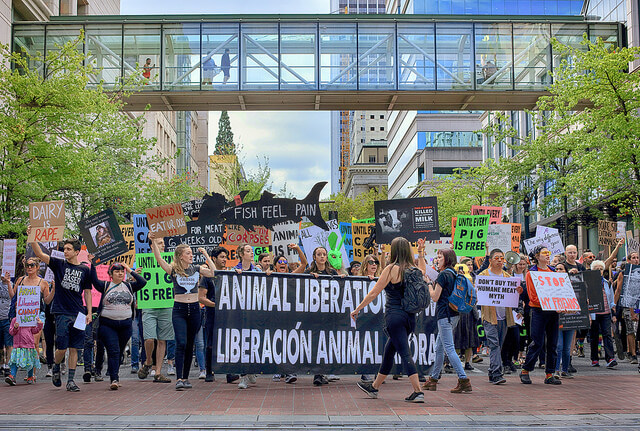
\includegraphics{assets/unit_7/U7_43699044114_5156812c09_z.jpg}

\emph{Image of animal liberation protest. Photo Credit: \href{https://flickr.com/photos/31246066}{flickr photo by Ian Sane}}

\hypertarget{overview-6}{%
\section*{Overview}\label{overview-6}}
\addcontentsline{toc}{section}{Overview}

Do animals have rights? We commonly speak of humans having rights, but animals? Could it be that your pet cat, or dog, or the local farmer's livestock, or even animals living in the wild, have rights to certain things? This question has been a point of intense discussion in the past few decades and it is the focus of this unit.
When we ask if animals have rights, we are really asking whether animals are the kinds of beings that could have rights. Of course, we cannot answer that question without having some idea of what kinds of beings have rights in the first place. If we can provide an answer to this question, then we will be well on our way to knowing whether animals have rights.
The question of whether animals have rights leads directly to a more foundational one, namely, what it means to attribute a right to a being, whether it be a human or an animal? What are we saying when we affirm that someone has a right to something?

A \textbf{right} is one of the strongest entities of which one could speak in both legal and moral discourse. It conveys the idea of being entitled to something. If a person does not receive something to which they have a right, then a wrong has been done. Their rights have been violated. This means that to affirm that one has a right to something is to make a forceful statement and one that carries implications for other people.

\textbf{Legal rights}, such as the right to live free of a home invasion, are declared and enforced by governments. If someone violates your legal rights by breaking into your home and robbing you at gun point, that person violates this legal right of yours. He has acted illegally and, consequently, if caught, will be subject to a penalty from the government.

In this unit, we are primarily concerned with moral rights rather than legal ones. \textbf{Moral rights} exist whether or not they are declared, recognized, or enforced by governments. Of course, there is often debate about whether something actually is a moral right, but few people disagree that moral rights exist.
To have a moral right to something, say a right to live free of harm from others, means one is entitled to live without being attacked by others in one's society regardless of whether the law requires it or not. If your neighbour attacks you in front of your home, then a moral wrong has been done since you did not receive something to which you had a moral right, namely an existence free of harm from others.

We can take this one step further. If you have a moral right to something, say to live in safety, it also means that someone somewhere, in this case other members of your society, have a corresponding \textbf{moral duty} to honour that right by not causing you harm. If they do, then they have not fulfilled their moral duty to you. They have acted immorally.

It should be obvious that the way we answer our original question of whether animals have rights will have a far-reaching implication for us. If we affirm that animals do have rights, it will mean that we have corresponding duties to treat them in certain ways and, in fact, are acting immorally if we do not treat them in these ways.
We may prefer to deny that animals have rights in order to relieve ourselves of our duties toward them. Our desire to avoid moral duties, however, will not count as a legitimate reason for a no-animal-rights position because moral rights, by their nature, are not things we simply decide to confer upon others. That's how legal rights work, but not moral rights. Moral rights are entities we simply recognize or discover.

If animals do have rights, then a few other questions immediately follow. Which animals, what rights, and how did they get them? What is the basis for believing such rights exist?
To answer this, we could ask how we, as humans, ``get'' the rights we say we have, rights to such things as life and liberty. Legal rights come from the government, but from where do we derive moral rights? Answering this question will inevitably lead to the question of what kinds of beings have rights.
A more technical way of asking this is: \textbf{What are the ``rights-giving characteristics'' which any being who has rights possesses, and do any animals possess these characteristics?} This, then, becomes one of the key questions for us to explore. Answering it will help us determine whether a particular animal has rights. Different answers have been given to this query and we will see three very different ones in the readings for this unit.
We will have an opportunity to examine and evaluate the basis for different perspectives regarding our duties to animals with our class colleagues.

\hypertarget{topics-6}{%
\subsection*{Topics}\label{topics-6}}
\addcontentsline{toc}{subsection}{Topics}

This unit is divided into 3 topics:

\begin{enumerate}
\def\labelenumi{\arabic{enumi}.}
\tightlist
\item
  Are Animals Self-Aware?\\
\item
  Do We Practice Speciesism?\\
\item
  Animals Do Have Rights But. . .
\end{enumerate}

\hypertarget{learning-outcomes-6}{%
\subsection*{Learning Outcomes}\label{learning-outcomes-6}}
\addcontentsline{toc}{subsection}{Learning Outcomes}

When you have completed this unit you should be able to:

\begin{itemize}
\tightlist
\item
  Define the term ``right.''\\
\item
  Specify the difference between legal and moral rights.\\
\item
  Explain how moral rights are related to moral duties.\\
\item
  Identify at least two rights-giving-characteristics which any being which possesses moral rights must have.\\
\item
  Explain and assess Peter Singer's rationale for his view that animals have certain moral rights.
\end{itemize}

\hypertarget{activity-checklist-6}{%
\subsection*{Activity Checklist}\label{activity-checklist-6}}
\addcontentsline{toc}{subsection}{Activity Checklist}

Here is a checklist of learning activities you will benefit from in completing
this unit. You may find it useful for planning your work.

\begin{reflect}
\hypertarget{read-view-and-reflect-20}{%
\subsubsection*{Read, View and Reflect}\label{read-view-and-reflect-20}}
\addcontentsline{toc}{subsubsection}{Read, View and Reflect}

\begin{itemize}
\tightlist
\item
  Read the introductory section on animal rights (pages 426-27) and the section by Immanuel Kant (p.~428-29) in your \emph{Readings} textbook. Watch the videos related to the topic.\\
\item
  Read the section on animal rights by Peter Singer (pages 429-435) in your \emph{Readings} textbook. Watch the videos related to the topic.\\
\item
  Read the section on animal rights by Roger Scruton (pages 436-443) in your \emph{Readings} textbook. Watch the videos related to the topic.
\end{itemize}

\hypertarget{singer-case-study}{%
\subsubsection*{Singer Case Study}\label{singer-case-study}}
\addcontentsline{toc}{subsubsection}{Singer Case Study}

Read and analyze the case study presented.

\hypertarget{ai-extension}{%
\subsubsection*{AI Extension}\label{ai-extension}}
\addcontentsline{toc}{subsubsection}{AI Extension}

Read an article and watch the video on AI and personhood. Reflect on if AI should have rights.

\hypertarget{key-terms-quiz-5}{%
\subsubsection*{Key Terms Quiz}\label{key-terms-quiz-5}}
\addcontentsline{toc}{subsubsection}{Key Terms Quiz}

Take the ungraded quiz to review important concepts.

\hypertarget{assignment-4}{%
\subsubsection*{\texorpdfstring{\textbf{Assignment}}{Assignment}}\label{assignment-4}}
\addcontentsline{toc}{subsubsection}{\textbf{Assignment}}

Ethics Committee Response (15\%)
\end{reflect}

\hypertarget{resources-6}{%
\subsection*{Resources}\label{resources-6}}
\addcontentsline{toc}{subsection}{Resources}

Here are the resources you will need to complete this unit.

\begin{itemize}
\tightlist
\item
  Wolff, Jonathan. ~\emph{Readings in Moral Philosophy}. ~New York: W. W. Norton \& Company, 2018.\\
\item
  Other online resources will be provided in the unit.
\end{itemize}

\hypertarget{are-animals-self-aware}{%
\section*{Are Animals Self-Aware?}\label{are-animals-self-aware}}
\addcontentsline{toc}{section}{Are Animals Self-Aware?}

The first answer concerning animal rights that we will consider is given by the eighteenth century German philosopher, Immanuel Kant, who believed animals do not have rights. Interestingly he tied his answer directly to the question of what kinds of being have rights. In order to have a right, says Kant, a being must be self-conscious, or in other words, self-aware. Since he believed animals do not have this characteristic, they cannot possess rights.
As we read his article, we will want to note carefully how he arrived at these two conclusions, first, that a key rights-giving characteristic of any being is self-consciousness (sometimes referred to as self-awareness), and secondly, that animals do not possess this characteristic.
Let's suppose, for purposes of argument, that Kant was correct. What does this mean, then, for the way we should treat animals? One might think that if animals have no rights, as Kant argued, that we are free to treat them in just any old way. We may be surprised at Kant's answer to this question but it is one to which we will also want to pay special attention. Once we understand it, we will be in a position to see if we agree with it.

\hypertarget{learning-activities-16}{%
\subsection*{Learning Activities}\label{learning-activities-16}}
\addcontentsline{toc}{subsection}{Learning Activities}

\begin{reflect}
\hypertarget{read-view-and-reflect-21}{%
\subsubsection*{Read, View and Reflect}\label{read-view-and-reflect-21}}
\addcontentsline{toc}{subsubsection}{Read, View and Reflect}

In the first activity, you are asked to read the introductory section on animal
rights (pages 426-27) and the section by Immanuel Kant (p.~428-29) in your
textbook, \emph{Readings in Moral Philosophy} by Jonathan Wolff. As you read, take
notes in your Learning Journal, defining key terms and explaining key concepts.
Next, choose from the following videos to learn more about key terms from this
topic.
\end{reflect}

\hypertarget{do-we-practice-speciesism}{%
\section*{Do We Practice Speciesism?}\label{do-we-practice-speciesism}}
\addcontentsline{toc}{section}{Do We Practice Speciesism?}

The second answer to our question about animal rights could hardly be more different from Immanuel Kant's. It comes from well-known American ethicist, Peter Singer, who argued that animals do, indeed, have rights, in the same strong sense as we humans have them. Furthermore, since animals have rights, it means that many of our current practices involving animals are actually immoral. They violate the rights of animals.
In fact, Singer went so far as to argue that the very principle of equality which we apply to humans should be extended to many animals as well. When we restrict this principle to humans, he said, we are guilty of something he called \textbf{speciesism}.
While this term may be new to us, it is one we will want to understand clearly when we read his article. It is akin to the terms, racism and sexism, which refer to practices which are immoral because they violate the principle of equality. Speciesism, said Singer, also violates this principle and, for this reason, is immoral as well.
As we read through Singer's article, we'll want to see precisely what he meant by the term, speciesism, and how he reasoned to his conclusion that animals have rights in this strong sense.

\hypertarget{learning-activities-17}{%
\subsection*{Learning Activities}\label{learning-activities-17}}
\addcontentsline{toc}{subsection}{Learning Activities}

\begin{reflect}
\hypertarget{read-view-and-reflect-22}{%
\subsubsection*{Read, View and Reflect}\label{read-view-and-reflect-22}}
\addcontentsline{toc}{subsubsection}{Read, View and Reflect}

Read the section on animal rights by Peter Singer (pages 429-435) in your textbook, \emph{Readings in Moral Philosophy} by Jonathan Wolff. Take notes defining key terms and ideas. Study the chapter review summary, questions and key terms.
Next, choose from the following videos to learn more about key terms from this topic.
\end{reflect}

\hypertarget{animals-do-not-have-rights-but.-.-.}{%
\section*{Animals-Do-Not-Have-Rights-But. . .}\label{animals-do-not-have-rights-but.-.-.}}
\addcontentsline{toc}{section}{Animals-Do-Not-Have-Rights-But. . .}

The third answer to our question about animal rights comes from American English professor, Roger Scruton, and could be summed up as the, ``Animals-do-not-have-rights-but. . .'' position. They do not have rights, says Scruton, for the simple reason that they are not the kinds of beings that possess rights. Notice that in saying this, Scruton, like Kant, is grounding his view on animal rights directly in the question of the kind of beings which have rights.

What kinds of beings, then, do have rights? Scruton's answer is that \textbf{persons} have rights while \textbf{nonpersons} do not. But what, precisely, does it mean to be a person? It means, he says, that one has the distinguishing features of personhood which include such things as self-awareness, the power of reason, personality, etc. Persons are capable of entering into ongoing dialogue with other persons. To state this more technically, personhood is the chief rights-giving characteristic.

Scruton also introduces the term \textbf{moral community.} This refers to a group of persons who have both moral rights and also corresponding moral duties to each other. Again, they have these because they are the types of beings which are capable of having such rights and duties, namely, persons. Animals, on the other hand, are not members of moral communities since they do not have these characteristics.

As we read Scruton's article, we will want to ask, however, if he has left open the possibility that there could be exceptions to his principle. What would happen, for example, if we discovered animals that did appear to have these rights-giving characteristics, self-awareness, reason, personality, etc.? Might they be persons? If so, would we need to regard them as having rights and duties and, thus, as being members of a moral community?

Regardless of how we answer that question, we will also want to pay special heed to the question of how animals should be treated if they really have no rights, as Scruton argues. It's the same question we asked for Immanuel Kant's view. If they have no rights, does this mean that any treatment of them at all is morally permissible? Interestingly, Scruton's answer is, no. He argues that we still have moral duties to animals even though these duties are not grounded in any rights possessed by the animals. On what, then, are they grounded?

We will want to take special note of Scruton's reasoning and learn on what he is grounding our duties to animals. If they are not grounded on any rights possessed by the animals, then where do our duties come from? Once we grasp his answer to this question, we will be in a position to assess the basis he provides for our duties toward animals.

\hypertarget{learning-activities-18}{%
\subsection*{Learning Activities}\label{learning-activities-18}}
\addcontentsline{toc}{subsection}{Learning Activities}

\begin{reflect}
\hypertarget{read-view-and-reflect-23}{%
\subsubsection*{Read, View and Reflect}\label{read-view-and-reflect-23}}
\addcontentsline{toc}{subsubsection}{Read, View and Reflect}

Read the section on animal rights by Roger Scruton (pages 436-443) in your textbook, \emph{Readings in Moral Philosophy} by Jonathan Wolff. Take notes defining key terms and ideas. Study the chapter review summary, questions and key terms.
Next, watch the following videos to learn more about key terms from this topic.

\href{https://www.khanacademy.org/partner-content/wi-phi/wiphi-value-theory/wiphi-ethics/v/moral-status}{PHILOSOPHY - Ethics: Moral Status} (7 minutes)

\hypertarget{case-study}{%
\subsubsection*{Case Study}\label{case-study}}
\addcontentsline{toc}{subsubsection}{Case Study}

For this case study, analyze Peter Singer's well-known contention that the vital characteristic that gives a being the right to equal consideration is not the \textbf{ability to reason}, as is commonly assumed, but rather the \textbf{capacity for suffering.} To review this, see his article in the course readings (pages 429-432). ~Do you agree with this contention? Why or why not? State also whether you agree with the principle he derives from this contention, namely, that the principle of equality which we commonly apply to humans should be extended to other species. If you agree with this, explain why. If you do not agree, explain why. In either case, draw upon the concepts and principles from both Immanuel Kant's and Roger Scruton's articles.
\emph{Note that you may be asked to review this case or similar cases in your class discussion groups. You may want to prepare by relating the case to your readings. Specifically, identify the ethical issues and terms to help explain the case.}

\hypertarget{key-terms-quiz-ungraded-5}{%
\subsubsection*{Key Terms Quiz (ungraded)}\label{key-terms-quiz-ungraded-5}}
\addcontentsline{toc}{subsubsection}{Key Terms Quiz (ungraded)}

In order to review some of the major concepts from the text, take the following unmarked quiz. Although you will not be evaluated on these terms, they will assist you in the assignments for this course.
Match the following terms to their correct definition.

\hypertarget{artificial-intelligence-extension}{%
\subsubsection*{Artificial Intelligence Extension}\label{artificial-intelligence-extension}}
\addcontentsline{toc}{subsubsection}{Artificial Intelligence Extension}

There are many sci-fi movies and shows that play with the idea of the personhood of Artificial Intelligence. However, is this idea as fictional as it once was? Or has technological innovation brought this idea to the point where we need to seriously address it?

Watch the following video to learn more about if AI has rights. Then read the article from Forbes.

\href{https://www.forbes.com/sites/nicolemartin1/2019/02/08/did-a-robot-write-this-how-ai-is-impacting-journalism/\#6d4b9c347795}{Did A Robot Write This?}
\end{reflect}

\begin{caution}
\textbf{Questions to reflect on: }

How does some of the ideas surrounding the personhood of AI reflect some of the ideas and arguments you have encountered about animal rights?\\
What do you think? Could strong AI be considered a person and have rights? Use key terms from this unit to justify your answer.
\end{caution}

\hypertarget{assessment-6}{%
\section*{Assessment}\label{assessment-6}}
\addcontentsline{toc}{section}{Assessment}

\begin{assessment}
\hypertarget{assignment-ethics-committee-response-15}{%
\subsection*{Assignment: Ethics Committee Response (15\%)}\label{assignment-ethics-committee-response-15}}
\addcontentsline{toc}{subsection}{Assignment: Ethics Committee Response (15\%)}

After completing this unit, including the learning activities, you are asked to
meet with your Ethics Committee and create a response to the following:

A strongly worded editorial has just appeared in a local newspaper accusing the community zoo, and all zoos, of violating the rights of animals. Among other things, the author of the article pointedly asked, ``How would we like it if we were the ones being confined in this way? It's not natural for humans and it's not for animals either.''

A group is now lobbying the city council to shut down the zoo and the council has turned to your ethics committee for a recommendation. Your task is to write a brief report in which you do the following things:

\begin{itemize}
\tightlist
\item
  Define the concept of a right.\\
\item
  State whether or not animals have rights. Tell why you answer as you do.\\
\item
  If animals do have rights, does the practice of keeping them in zoos violate their rights. Again, give a reason for your answer.
\end{itemize}

As you collaborate on this assignment, be sure to refer to the \textbf{grading
criteria} in the Assessments section of this course. Submit your report on
Moodle by the end of the week.

\hypertarget{assignment-reflective-journal-ungraded-practice-2}{%
\subsection*{Assignment: Reflective Journal (ungraded practice)}\label{assignment-reflective-journal-ungraded-practice-2}}
\addcontentsline{toc}{subsection}{Assignment: Reflective Journal (ungraded practice)}

After completing this unit, including the learning activities, you are asked to
write a Reflective Journal entry of 250-400 words, answering the following:
Examine Peter Singer's basis for moral obligation to animals, including an analysis of Singer's extension of the principle of equality to animals. On what is this principle based? What does it mean to say animals are ``equal'' to humans?~ State your agreement or disagreement with this principle along with your reasons.
In addition, consider the issue of animal abuse. What steps could you take to solve this problem or advocate for animal rights?

\hypertarget{discussion-responses-2}{%
\subsection*{Discussion Responses}\label{discussion-responses-2}}
\addcontentsline{toc}{subsection}{Discussion Responses}

After you have finished your journal assignment, you will share your responses in class with your peers. As you discuss, be sure to respond substantively. Be sure to include your initial journal response, as well as ideas from your class discussion.
\end{assessment}

\hypertarget{checking-your-learning-6}{%
\section*{Checking your Learning}\label{checking-your-learning-6}}
\addcontentsline{toc}{section}{Checking your Learning}

\begin{progress}
Before you move on to the next unit, you may want to check to make sure that you are able to:

\begin{itemize}
\tightlist
\item
  Define the term ``right.''\\
\item
  Specify the difference between legal and moral rights.\\
\item
  Explain how moral rights are related to moral duties.\\
\item
  Identify at least two rights-giving-characteristics which any being which possesses moral rights must have.\\
\item
  Explain and assess Peter Singer's rationale for his view that animals have certain moral rights.
\end{itemize}
\end{progress}

\hypertarget{end-of-life-moral-dilemmas}{%
\chapter{End-of-Life Moral Dilemmas}\label{end-of-life-moral-dilemmas}}


\includegraphics{assets/unit_8/U8_hospice-1761276_1920.jpg}

\emph{image of an elderly man being cared. Photo Credit: \href{https://pixabay.com/en/hospice-caring-elderly-old-1761276/}{Pixabay}}

\hypertarget{overview-7}{%
\section*{Overview}\label{overview-7}}
\addcontentsline{toc}{section}{Overview}

Suppose one of your loved ones is on her death bed with no hope of recovery and has just slipped into a coma. Imagine also that the medical staff has come to you asking for direction as to how to proceed. They present you with a number of options. They could maintain your loved one's life for quite some time in this vegetative state or they could withdraw the life-saving equipment and allow your loved one to die probably in the next four to six hours. They could even administer a lethal injection and intentionally bring about the death of your loved one at the time of your choosing.

What should you do? Are you obligated, ethically, to use every medical means at your disposal to keep your loved one alive as long as possible? Or does there come a point when you are morally free to remove the life-saving technology and allow your loved one to die? If so, at what point does this become an ethically acceptable option and why? What basis is there for choosing this time as opposed to a few days earlier, or later?

To take this one step further, does there ever come a time when you are morally free, or even obligated, to ask the medical staff to administer a painless lethal injection and intentionally end the life of your loved one? Would this course of action be compatible with your desire to be charitable to your loved one, or with your deep respect for human dignity in general?

What if your loved one had previously asked you to have a lethal injection administered if she ever became unable to make her own life decisions? Does this change your moral obligation?

Welcome to unit eight. In this unit, we turn our attention to moral dilemmas like these, ones surrounding the end of life. Two things are immediately true of these dilemmas: first, they present some of the toughest choices many of us will make in our lives, and second, few of us will be able to avoid these choices forever. At some point, most of us will be called upon to make difficult decisions about end-of-life care for someone.

In end-of-life dilemmas, situations vary greatly and the details matter. The key question for us as we examine these situations from an ethical standpoint is whether there are any guiding principles which can be applied to these different situations to give us moral direction?

Cases like the one above are difficult. In this unit we will read about concepts like \textbf{voluntary euthanasia}, \textbf{nonvoluntary euthanasia}, \textbf{passive euthanasia}, and \textbf{active euthanasia}. It will be important to grasp how each of these concepts is similar to and yet distinct from the others.

This unit will also address another, very different, end-of-life ethical dilemma, namely the question of capital punishment. Rather than considering the best choice for a loved one on her death bed, we are now asking what, morally, should be done by the state to someone who has committed heinous crimes such as rape or murder.

Do principles of justice either allow or mandate the execution of such a person? Or do they rule out capital punishment as unjust and immoral in every situation? The way we decide these questions matters greatly to our world and we need to decide them on the basis of relevant moral principles.
Let's prepare for some moral choices we may well have to make in the future.

\hypertarget{topics-7}{%
\subsection*{Topics}\label{topics-7}}
\addcontentsline{toc}{subsection}{Topics}

This unit is divided into three topics:

\begin{enumerate}
\def\labelenumi{\arabic{enumi}.}
\tightlist
\item
  Active \& Passive Euthanasia\\
\item
  Capital Punishment: A Defense\\
\item
  How to Reason Ethically About Capital Punishment
\end{enumerate}

\hypertarget{learning-outcomes-7}{%
\subsection*{Learning Outcomes}\label{learning-outcomes-7}}
\addcontentsline{toc}{subsection}{Learning Outcomes}

When you have completed this unit you should be able to:

\begin{itemize}
\tightlist
\item
  Describe key concepts in the euthanasia discussion including euthanasia, active euthanasia, passive euthanasia, voluntary euthanasia, non-voluntary euthanasia, and killing versus letting die.\\
\item
  Explain James Rachels' moral equivalency argument concerning active euthanasia and passive euthanasia.\\
\item
  Articulate John Stuart Mill's case for the moral permissibility of capital punishment.\\
\item
  Discuss the strongest objections to the case for capital punishment.
\end{itemize}

\hypertarget{activity-checklist-7}{%
\subsection*{Activity Checklist}\label{activity-checklist-7}}
\addcontentsline{toc}{subsection}{Activity Checklist}

Here is a checklist of learning activities you will benefit from in completing this unit. You may find it useful for planning your work.

\begin{reflect}
\hypertarget{read-view-and-reflect-24}{%
\subsubsection*{Read, View and Reflect}\label{read-view-and-reflect-24}}
\addcontentsline{toc}{subsubsection}{Read, View and Reflect}

\begin{itemize}
\tightlist
\item
  Read the section on euthanasia by James Rachels (pages 372-378) and Philippa Foot (379-388) in your \emph{Readings} textbook. Watch the video related to the topic.\\
\item
  Read the section on capital punishment by John Stuart Mill (390-397) in your \emph{Readings} textbook. Watch the videos related to the topic.\\
\item
  Read the section on euthanasia by Hugo Adam Bedau (pages 397-406) in your \emph{Readings} textbook.
\end{itemize}

\hypertarget{smith-and-jones-case-study}{%
\subsubsection*{Smith and Jones Case Study}\label{smith-and-jones-case-study}}
\addcontentsline{toc}{subsubsection}{Smith and Jones Case Study}

Read and analyze the case study presented.

\hypertarget{key-terms-quiz-6}{%
\subsubsection*{Key Terms Quiz}\label{key-terms-quiz-6}}
\addcontentsline{toc}{subsubsection}{Key Terms Quiz}

Take the ungraded quiz to review important concepts.

\hypertarget{assignment-5}{%
\subsubsection*{\texorpdfstring{\textbf{Assignment}}{Assignment}}\label{assignment-5}}
\addcontentsline{toc}{subsubsection}{\textbf{Assignment}}

Reflective Journal (5\%)
\end{reflect}

\hypertarget{resources-7}{%
\subsection*{Resources}\label{resources-7}}
\addcontentsline{toc}{subsection}{Resources}

Here are the resources you will need to complete this unit.

\begin{itemize}
\tightlist
\item
  Wolff, Jonathan. ~\emph{Readings in Moral Philosophy}. ~New York: W. W. Norton \& Company, 2018.\\
\item
  Other online resources will be provided in the unit.
\end{itemize}

\hypertarget{active-passive-euthanasia}{%
\section*{Active \& Passive Euthanasia}\label{active-passive-euthanasia}}
\addcontentsline{toc}{section}{Active \& Passive Euthanasia}

\textbf{Active euthanasia} occurs when steps are taken to euthanize a person, perhaps by giving a lethal injection or an overdose of pain-killers. \textbf{Passive euthanasia} happens when life-saving medical equipment is either withheld or withdrawn from a person with the intention of letting that person die from their underlying disease or condition.
Are active and passive euthanasia morally equivalent to each other? In other words, is one of these just as good (or bad) as the other, or is one morally worse than the other? How does one decide a question like this?
Related to this question is the distinction between \textbf{killing} and \textbf{letting die}. Most of us would probably instinctively view killing as morally worse than letting die, but in the reading by American ethicist, James Rachels, we will have an opportunity to think through this question and test our moral intuitions.
If all other factors were the same, asks Rachels, such as our motives and purposes in acting, would killing a person be morally worse than letting that same person die? His answer may surprise you. The way we reply to this question will have far-reaching implications for our views concerning passive euthanasia and physician-assisted suicide.

\hypertarget{learning-activities-19}{%
\subsection*{Learning Activities}\label{learning-activities-19}}
\addcontentsline{toc}{subsection}{Learning Activities}

\begin{reflect}
\hypertarget{read-view-and-reflect-25}{%
\subsubsection*{Read, View and Reflect}\label{read-view-and-reflect-25}}
\addcontentsline{toc}{subsubsection}{Read, View and Reflect}

In the first activity, you are asked to read the section on euthanasia by James Rachels (pages 372-378) and Philippa Foot (379-388) in your textbook, \emph{Readings in Moral Philosophy} by Jonathan Wolff. As you read, take notes in your Learning Journal, defining key terms and explaining key concepts.
Next, choose from the following videos to learn more about key terms from this
topic.
\end{reflect}

\begin{caution}
\textbf{Note} that the first part of the video focusses on abortion, but it relevant to the discussion on euthanasia. If you prefer to skip ahead, go to 6:42 minute mark for euthanasia-specific content.
\end{caution}

\hypertarget{capital-punishment-a-defense}{%
\section*{Capital Punishment: A Defense}\label{capital-punishment-a-defense}}
\addcontentsline{toc}{section}{Capital Punishment: A Defense}

The issue of capital punishment presents us with a starkly different kind of end-of-life ethical question. We are no longer considering our best course of action toward our loved ones who are suffering or dying. Rather we are asking how someone who has committed vile crimes should be treated by their governments.
Specifically, we are asking whether there are cases in which justice would allow for, or even require, a state to execute such a person. The challenge for all of us is to move beyond how we may feel toward people who have committed atrocious crimes, especially if they were against one of our loved ones, and ask if principles of justice would call for their execution.
We will read a well-known case in favour of capital punishment by John Stuart Mill who argues on utilitarian grounds that having this option available will lead to better consequences for a society than ruling it out. It will be important for us to consider his arguments and see whether we agree with him or not.
\#\#\# Learning Activities \{-\}

\begin{reflect}
\hypertarget{read-view-and-reflect-26}{%
\subsection*{Read, View and Reflect}\label{read-view-and-reflect-26}}
\addcontentsline{toc}{subsection}{Read, View and Reflect}

\begin{itemize}
\tightlist
\item
  Read the section on capital punishment by John Stuart Mill (390-397) in your textbook, \emph{Readings in Moral Philosophy} by Jonathan Wolff.\\
\item
  Take notes defining key terms and ideas. Study the chapter review summary, questions and key terms.\\
\item
  Next, choose from the following videos to learn more about key terms from this topic.
\end{itemize}
\end{reflect}

\hypertarget{how-to-reason-ethically-about-capital-punishment}{%
\section*{How to reason ethically about Capital Punishment}\label{how-to-reason-ethically-about-capital-punishment}}
\addcontentsline{toc}{section}{How to reason ethically about Capital Punishment}

In the previous topic, we learned how one thinker reasons in defense of capital punishment. Could it be, however, that neither side on this issue has conclusive arguments. That is the view of Hugo Bedau, an American political philosopher who has written an article we will read for this topic.
How, then, should one proceed in figuring out this issue? Bedau contends that, since neither those who argue \textbf{for} or \textbf{against} bring overwhelming supporting arguments, a better way forward is to shift our focus to the \textbf{goals} of punishment in the first place.
In other words, according to Bedau, the first question to ask is not whether capital punishment is ever morally justified, but rather, \textbf{what we are trying to accomplish by punishing} those who have committed vile crimes. Why do we punish them? What do we hope will be the outcome of our punishment? Different answers may be given to this question. Let's read Bedau's article to see how he answers it, and then see if this provides help in answering the larger question concerning the morality of capital punishment.

\hypertarget{learning-activities-20}{%
\subsection*{Learning Activities}\label{learning-activities-20}}
\addcontentsline{toc}{subsection}{Learning Activities}

\begin{reflect}
\hypertarget{read-view-and-reflect-27}{%
\subsubsection*{Read, View and Reflect}\label{read-view-and-reflect-27}}
\addcontentsline{toc}{subsubsection}{Read, View and Reflect}

Read the section on euthanasia by Hugo Adam Bedau (pages 397-406) in your
textbook, \emph{Readings in Moral Philosophy} by Jonathan Wolff. Take notes defining
key terms and ideas. Study the chapter review summary, questions and key terms.

\hypertarget{key-terms-quiz-ungraded-6}{%
\subsubsection*{Key Terms Quiz (ungraded)}\label{key-terms-quiz-ungraded-6}}
\addcontentsline{toc}{subsubsection}{Key Terms Quiz (ungraded)}

In order to review some of the major concepts from the text, take the following unmarked quiz. Although you will not be evaluated on these terms, they will assist you in the assignments for this course.
Match the following terms to their correct definition.

\hypertarget{case-study-1}{%
\subsubsection*{Case Study}\label{case-study-1}}
\addcontentsline{toc}{subsubsection}{Case Study}

Read the following case study and consider the questions presented.
Analyze James Rachels' `Smith and Jones' example from his article in the course readings. ~Drawing upon the arguments from all the readings for this unit, tell whether you agree with his conclusion that this example shows that in cases like this, killing a person is no worse morally than letting that same person die, that these two actions are morally equivalent? ~Why or why not? Then explain why Don Marquis would probably disagree with Rachels' conclusion.
\end{reflect}

\begin{caution}
\textbf{Note} that you may be asked to review this case or similar cases in your class discussion groups. You may want to prepare by relating the case to your readings. Specifically, identify the ethical issues and terms to help explain the case.
\end{caution}

\hypertarget{assessment-7}{%
\section*{Assessment}\label{assessment-7}}
\addcontentsline{toc}{section}{Assessment}

\begin{assessment}
\hypertarget{assignment-reflective-journal-5}{%
\subsubsection*{Assignment: Reflective Journal (5\%)}\label{assignment-reflective-journal-5}}
\addcontentsline{toc}{subsubsection}{Assignment: Reflective Journal (5\%)}

After completing this unit, including the learning activities, you are asked to write about what you have learned in this unit.
State John Stuart Mill's case for the moral permissibility of capital punishment and show how it grows out of his utilitarian perspective. ~Then explain a number of questions Hugo Bedau would raise about the argument made by Mill. Tell why, in the end, he would favour the abolition of capital punishment. ~Finally, discuss which view, Bedau's or Mill's, you would prefer and why.

\hypertarget{discussion-responses-3}{%
\subsubsection*{Discussion Responses}\label{discussion-responses-3}}
\addcontentsline{toc}{subsubsection}{Discussion Responses}

After you have finished your journal assignment, you will share your responses in class with your peers. Refer to the \textbf{grading criteria} in the Assessments section of this course. Be sure to include your initial journal response, as well as ideas from your class discussion. Submit your assignment on Moodle by the end of the week.
\end{assessment}

\hypertarget{checking-your-learning-7}{%
\section*{Checking your Learning}\label{checking-your-learning-7}}
\addcontentsline{toc}{section}{Checking your Learning}

\begin{progress}
Before you move on to the next unit, you may want to check to make sure that you
are able to:

\begin{itemize}
\tightlist
\item
  Describe key concepts in the euthanasia discussion including euthanasia, active euthanasia, passive euthanasia, voluntary euthanasia, non-voluntary euthanasia, and killing versus letting die.\\
\item
  Explain James Rachels' moral equivalency argument concerning active euthanasia and passive euthanasia.\\
\item
  Articulate John Stuart Mill's case for the moral permissibility of capital punishment.\\
\item
  Discuss the strongest objections to the case for capital punishment.
\end{itemize}
\end{progress}

\hypertarget{the-ethics-of-torture-and-terrorism}{%
\chapter{The Ethics of Torture and Terrorism}\label{the-ethics-of-torture-and-terrorism}}


\includegraphics{assets/unit-9/U9_chair-3624563_1920.jpg}

\emph{image of a broken saloon chair. Photo Credit: \href{https://pixabay.com/en/chair-seat-treatment-interrogation-3624563/}{Pixabay}}

\hypertarget{overview-8}{%
\section*{Overview}\label{overview-8}}
\addcontentsline{toc}{section}{Overview}

Welcome to Unit 9. In this unit we will be addressing a harsh and disquieting topic, namely torture and terrorism. Perhaps you've never thought of this as an issue open to ethical discussion. It's just bad people and corrupt governments who use torture techniques, isn't it, so what is there to discuss about the ethics of this practice?

That's a fair question. This topic has not been part of the normal civilized discourse for a few centuries now. A few recent events, however, have moved it into the realm of discussion and it has, for better or worse, become a topic no one can avoid in the worlds of ethics and politics.

Torture, in the sense we will use it in this unit, involves \textbf{inflicting pain or suffering on a person by the state for the purpose of extracting information}. The usual justification offered is that this information could, conceivably, be useful in saving other human lives. In our reading by Alan Dershowitz, American lawyer and Harvard University professor emeritus, we will see a fuller definition which contains these same elements.

The ethical question we will face is whether we are ever morally justified in supporting our governments to carry out this practice. Imagine a government in possession of people who may have information which could be useful in preventing the suffering or deaths of many more people. Remember the people who may be tortured need not be guilty of any wrong doing. Their only ``offence'' is having information that a particular government believes could conceivably be useful in saving other lives.

To take a real-life example, in 1978, would the government of Italy have been justified in using torturous interrogation methods on a person in their possession to try to gain information which could possibly have led to the release of their former prime minister who had been captured by terrorists? The Italian police chose not to use such methods, believing their country could not withstand the introduction of torture to their culture. The prime minister was later executed by his captors. Or another: would the government of the United States be justified in using torture techniques today to try prevent a recurrence of 9/11?

In our second reading, by Michael Walzer, an American political philosopher who has worked a great deal on issues of social justice, we will shift our focus to the issue of terrorism. Once again, many of us have never considered terrorism to be an issue which is up for ethical discussion. Terrorism is evil, pure and simple, isn't it? What's there to discuss about the ethics of terrorism? Interestingly, arguments and reasons have been offered in support of acts of terrorism in certain cases and Walzer presents a number of them in his article. Once we understand these arguments, we will be in a position to evaluate them.

For instance, in both readings for this unit, we will see that the utilitarian argument in favour of torture is that it has the potential to save many lives and prevent much suffering by causing the suffering of only one person. We will have opportunities to discuss this argument and others, too, with our class colleagues to determine if there are any problems with them.
Let's prepare for some fascinating reading and lively discussion on an intense current social issue.

\hypertarget{topics-8}{%
\subsection*{Topics}\label{topics-8}}
\addcontentsline{toc}{subsection}{Topics}

This unit is divided into two topics:

\begin{enumerate}
\def\labelenumi{\arabic{enumi}.}
\tightlist
\item
  Is Torture ever Justified? ~
\item
  A Rationale for Terrorism: A Response. ~
\end{enumerate}

\hypertarget{learning-outcomes-8}{%
\subsection*{Learning Outcomes}\label{learning-outcomes-8}}
\addcontentsline{toc}{subsection}{Learning Outcomes}

When you have completed this unit you should be able to:

\begin{itemize}
\tightlist
\item
  Define key terms in the discussions of torture and terrorism including lethal versus non-lethal torture, ``ticking bomb'' cases, coercive interrogation, and terrorism.\\
\item
  Explain how Alan Dershowitz's view permitting torture in certain cases arises from a utilitarian perspective.\\
\item
  Describe how the question of torture pits certain widely held values against each other.\\
\item
  State a rationale terrorists often use to justify their actions.\\
\item
  Discuss objections to this terrorist rationale.
\end{itemize}

\hypertarget{activity-checklist-8}{%
\subsection*{Activity Checklist}\label{activity-checklist-8}}
\addcontentsline{toc}{subsection}{Activity Checklist}

Here is a checklist of learning activities you will benefit from in completing this unit. You may find it useful for planning your work.

\begin{reflect}
\hypertarget{read-view-and-reflect-28}{%
\subsubsection*{Read, View and Reflect}\label{read-view-and-reflect-28}}
\addcontentsline{toc}{subsubsection}{Read, View and Reflect}

\begin{itemize}
\tightlist
\item
  Read the section on terror and torture by Alan Dershowitz (pages 488-501) in your \emph{Readings} textbook. Watch the videos related to the topic.\\
\item
  Read the section on terror and torture by Michael Walzer (pages 501-511) in your \emph{Readings} textbook. Watch the videos related to the topic.
\end{itemize}

\hypertarget{current-event-search}{%
\subsubsection*{Current Event Search}\label{current-event-search}}
\addcontentsline{toc}{subsubsection}{Current Event Search}

Look up current events regarding torture and terrorism.

\hypertarget{key-terms-quiz-7}{%
\subsubsection*{Key Terms Quiz}\label{key-terms-quiz-7}}
\addcontentsline{toc}{subsubsection}{Key Terms Quiz}

Take the ungraded quiz to review important concepts.

\hypertarget{assignment-6}{%
\subsubsection*{\texorpdfstring{\textbf{Assignment}}{Assignment}}\label{assignment-6}}
\addcontentsline{toc}{subsubsection}{\textbf{Assignment}}

Ethics Video (15\%)
\end{reflect}

\hypertarget{resources-8}{%
\subsection*{Resources}\label{resources-8}}
\addcontentsline{toc}{subsection}{Resources}

Here are the resources you will need to complete this unit.

\begin{itemize}
\tightlist
\item
  Wolff, Jonathan.~\emph{Readings in Moral Philosophy}. ~New York: W. W. Norton \& Company, 2018.\\
\item
  Other online resources will be provided in the unit.
\end{itemize}

\hypertarget{is-torture-ever-justified}{%
\section*{Is Torture Ever Justified?}\label{is-torture-ever-justified}}
\addcontentsline{toc}{section}{Is Torture Ever Justified?}

Are governments ever justified in using torture? Are we, as citizens, ever justified in supporting them in using torturous methods? In all ethical questions, facts matter greatly and this issue is no exception. Here are a few facts which are often raised in discussing this issue.

First, many countries signed the Geneva Convention in the mid-1980s which bans torture in all forms, and yet a good number of them continue to practice or use severe forms of torture anyway. In other words, hypocrisy on this issue is rampant. To make matters worse, since it is in violation of the convention, the torture is going on behind closed doors, unacknowledged, so there are no controls.

A second fact: As Alan Dershowitz points out in the article we will read by him, if a terrorist attack like 9/11 happened, and it was later revealed that the police had deliberately refused to take action that might have prevented the attack, including torture, there would be a great outcry.

One final unsettling fact is that, while it is commonly asserted that torture does not ``work'' because people will say anything to end the torture, Dershowitz highlights examples of where it has been successful in extracting useful information which has saved innocent civilians. This, he says, is precisely why a good number of countries continue to use it and, even those which say they do not, often utilize other countries as third parties to carry out torturous interrogations.

Do these facts make a difference in our ethical analysis of this question? If torture is happening anyway, and would, in certain cases, be desired by the general public, is it ethically preferable, as some argue, to legalize this practice, bring it out into the open, and place some controls on it? Is this what we should be encouraging our governments to do?

Furthermore, does it make a difference whether it works or not, whether it can successfully extract information which may save other lives? If it does not matter, why then do people who oppose torture often argue that it doesn't work? Proper ethical inquiry must apply rigorous reasoning in analyzing these facts.

These facts lead people to take differing opinions on this issue. As we read the article by Alan Derschowitz, we'll have an opportunity to engage with a number of the questions and arguments often expressed in both defending and criticizing the use of torture.

\hypertarget{learning-activities-21}{%
\subsection*{Learning Activities}\label{learning-activities-21}}
\addcontentsline{toc}{subsection}{Learning Activities}

\begin{reflect}
\hypertarget{read-view-and-reflect-29}{%
\subsubsection*{Read, View and Reflect}\label{read-view-and-reflect-29}}
\addcontentsline{toc}{subsubsection}{Read, View and Reflect}

In the first activity, you are asked to read the section on terror and torture by Alan Dershowitz (pages 488-501) in your textbook, \emph{Readings in Moral Philosophy} by Jonathan Wolff. As you read, take notes in your Learning Journal, defining key terms and explaining key concepts.
Next, view the following resources to learn more about key terms from this topic.

\href{https://ethicsunwrapped.utexas.edu/america-awesome-right}{America is Awesome\ldots Right?!}
\end{reflect}

\hypertarget{a-rationale-for-terrorism-a-response}{%
\section*{A Rationale for Terrorism: A Response}\label{a-rationale-for-terrorism-a-response}}
\addcontentsline{toc}{section}{A Rationale for Terrorism: A Response}

In this topic, we are shifting focus from torture to terrorism and this raises an immediate question: Isn't terrorism simply evil through and through? Shouldn't people who commit acts of terrorism be caught and locked up, and shouldn't that be the end of the matter? If so, then why are we discussing this issue in a course on ethics? What is there to discuss about the ethics of this practice?
Surprisingly, certain people have offered justifications for acts of terrorism under certain conditions, complete with arguments and lines of reasoning. In this topic, we will have an opportunity to acquaint ourselves with some of them through reading an article by Michael Walzer, an American political philosopher who has worked a great deal on issues of social justice. In this article, he has articulated a number of the arguments that are sometimes offered in support of certain acts of terrorism along with his own critiques of them. Once we have understood them, we'll be in a position to assess them.

\hypertarget{learning-activities-22}{%
\subsection*{Learning Activities}\label{learning-activities-22}}
\addcontentsline{toc}{subsection}{Learning Activities}

\begin{reflect}
\hypertarget{read-view-and-reflect-30}{%
\subsubsection*{Read, View and Reflect}\label{read-view-and-reflect-30}}
\addcontentsline{toc}{subsubsection}{Read, View and Reflect}

Read the section on terror and torture by Michael Walzer (pages 501-511) in your textbook, \emph{Readings in Moral Philosophy} by Jonathan Wolff. Take notes defining key terms and ideas. Study the chapter review summary, questions and key terms.
Next, choose from the following videos to learn more about key terms from this topic.

//todo \#3

//todo \#4

//todo \#5

\hypertarget{current-events}{%
\subsubsection*{Current Events}\label{current-events}}
\addcontentsline{toc}{subsubsection}{Current Events}

Go online and search for one or two current incidents involving torture. Next, apply the principles gained from both readings to these situations. Finally, consider whether you believe the torture used was ethically justified and give reasons for your position. Write your thoughts in your notes and review them as you complete the assessment for this unit.

\hypertarget{key-terms-quiz-ungraded-7}{%
\subsubsection*{Key Terms Quiz (ungraded)}\label{key-terms-quiz-ungraded-7}}
\addcontentsline{toc}{subsubsection}{Key Terms Quiz (ungraded)}

In order to review some of the major concepts from the text, take the following unmarked quiz. Although you will not be evaluated on these terms, they will assist you in the assignments for this course.
Match the following terms to their correct definition.
\end{reflect}

\hypertarget{assessment-8}{%
\section*{Assessment}\label{assessment-8}}
\addcontentsline{toc}{section}{Assessment}

\begin{assessment}
\hypertarget{assignment-reflective-journal-ungraded-practice-3}{%
\subsubsection*{Assignment: Reflective Journal (ungraded practice)}\label{assignment-reflective-journal-ungraded-practice-3}}
\addcontentsline{toc}{subsubsection}{Assignment: Reflective Journal (ungraded practice)}

After completing this unit, including the learning activities, you are asked to write about what you have learned in this unit. Remember that you should consider your journal as a place for you to try out new ideas, to test your assumptions, and to share what you are learning with your community.
Write a 250-400 word journal response discussing the reasons Alan Dershowitz believes that, in certain cases, torture is morally permissible when carried out under rigorous regulations. ~Then show how he believes his view follows from a utilitarian perspective. Following that, analyze his view and formulate two searching questions you think he would need to answer to defend his view further. ~Finally, tell how you think a different utilitarian thinker could argue against the moral permissibility of torture?

\hypertarget{discussion-responses-4}{%
\subsubsection*{Discussion Responses}\label{discussion-responses-4}}
\addcontentsline{toc}{subsubsection}{Discussion Responses}

After you have finished your journal assignment, you will share your responses in class with your peers. As you discuss, be sure to respond substantively.

\hypertarget{assignment-ethics-video-15}{%
\subsection*{Assignment: Ethics Video (15\%)}\label{assignment-ethics-video-15}}
\addcontentsline{toc}{subsection}{Assignment: Ethics Video (15\%)}

This video must be posted on Moodle by the end of week 9. ~If you choose to post it online outside of Moodle (e.g.~YouTube), please provide the URL. \textbf{You will write 3 posts (150 words each) responding to three videos presented by your classmates, stating your agreement or disagreement with the arguments in the video, and explaining why you agree or disagree.} Refer to the assignment details and \textbf{grading criteria} in the Assessments section of this course.
\end{assessment}

\hypertarget{checking-your-learning-8}{%
\section*{Checking your Learning}\label{checking-your-learning-8}}
\addcontentsline{toc}{section}{Checking your Learning}

\begin{progress}
Before you move on to the next unit, you may want to check to make sure that you
are able to:

\begin{itemize}
\tightlist
\item
  Define key terms in the discussions of torture and terrorism including lethal versus non-lethal torture, ``ticking bomb'' cases, coercive interrogation, and terrorism.\\
\item
  Explain how Alan Dershowitz's view permitting torture in certain cases arises from a utilitarian perspective.\\
\item
  Describe how the question of torture pits certain widely held values against each other.\\
\item
  State a rationale terrorists often use to justify their actions.\\
\item
  Discuss objections to this terrorist rationale.
\end{itemize}
\end{progress}

\hypertarget{world-hunger-and-foreign-aid}{%
\chapter{World Hunger and Foreign Aid}\label{world-hunger-and-foreign-aid}}

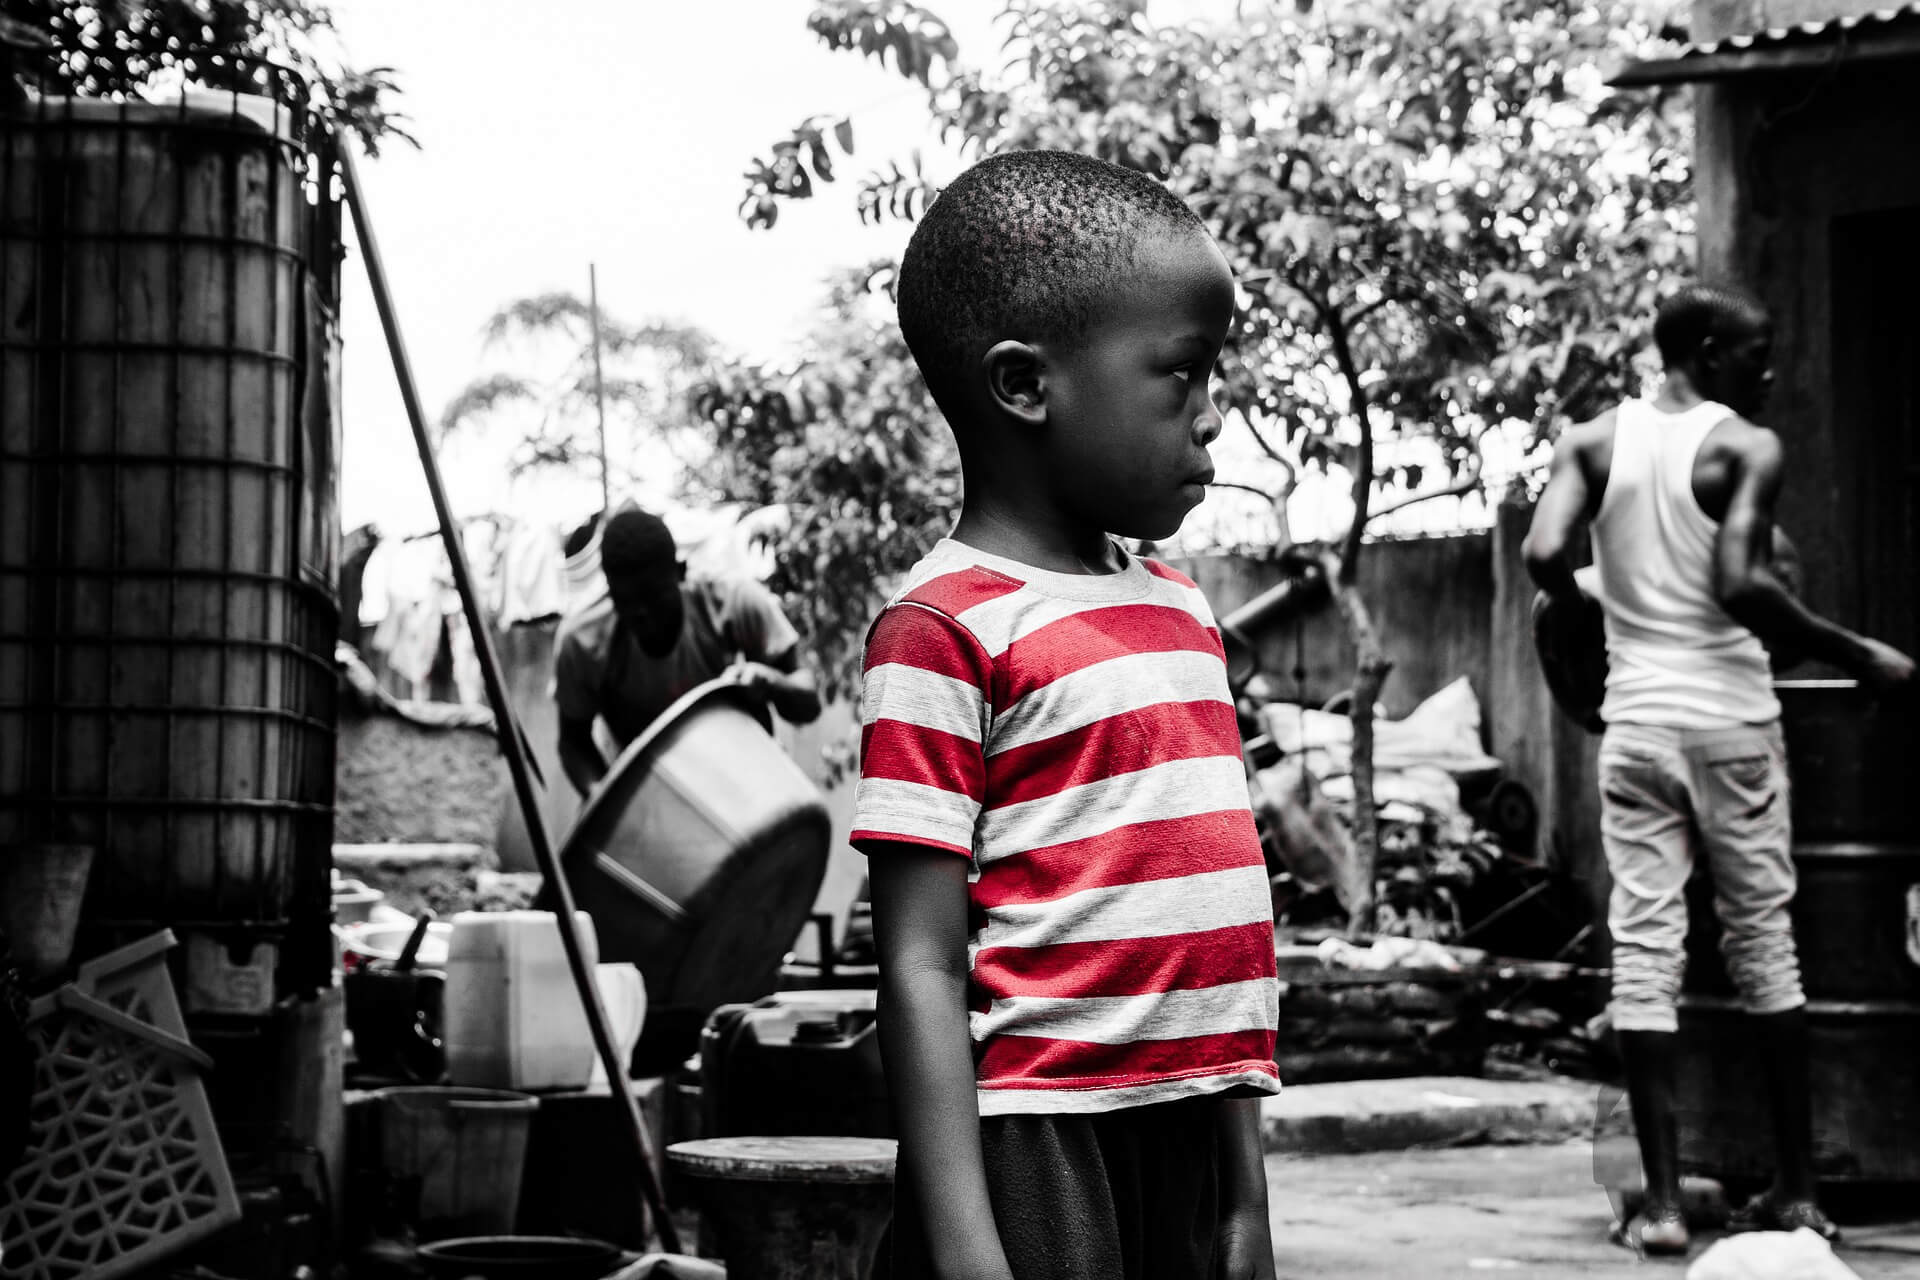
\includegraphics{assets/unit_10/U10_kid-2101832_1920.jpg}

\emph{image of a child looking away. Photo Credit: \href{https://pixabay.com/en/kid-child-sad-red-stripe-shirt-2101832/}{Pixabay}}

\hypertarget{overview-9}{%
\section*{Overview}\label{overview-9}}
\addcontentsline{toc}{section}{Overview}

Do people in prosperous countries have a moral obligation to provide help to other people in parts of the world where they do not have their basic needs satisfied? If so, why, and how should they carry out this moral obligation?

Clearly there are some people in the world, many people, who \emph{could} send food, clothing, money, medical equipment, etc., to others who do not have enough to survive on their own. This situation forces an ethical question upon us all: \textbf{If people can help in these ways, should they?} In other words, if people are \emph{able} to help, are they, thereby, morally \emph{obligated} to do so? Or is there no such moral obligation? Could it even be, as some argue, that we are morally required \emph{not} to help, at least in ways that some people think we are?

The way we answer this question has some rather serious and unavoidable implications. If we answer, that we are, indeed, morally obligated to help if we can, we are then affirming that if people who can help do \emph{not} do so, they are thereby acting immorally. They are violating their moral obligations in this regard.

Other questions immediately come to mind too. Does it matter if those in need are related to us, or known to us, or if they live close by, or happen to be in distant countries? Would it affect our moral obligations if there are other people who could be helping those in need but aren't? Is our moral obligation dependent upon factors like distance, relationships, other people's actions, etc., or does it stand completely independent of them?

In this unit we will become acquainted with three very different viewpoints on this question. This will provide us an opportunity to compare these different perspectives and assess them. Which one, or ones, do we agree with, and why? Is one ethically superior to the others? Again, why? To evaluate the various perspectives, we will first need to understand and evaluate the \emph{basis} for each.

\hypertarget{topics-9}{%
\subsection*{Topics}\label{topics-9}}
\addcontentsline{toc}{subsection}{Topics}

This unit is divided into 3 topics:

\begin{enumerate}
\def\labelenumi{\arabic{enumi}.}
\tightlist
\item
  A Proposed Basis for Moral Obligation\\
\item
  Does our aid help or hurt?\\
\item
  How to Think about Moral Obligation to those in need.
\end{enumerate}

\hypertarget{learning-outcomes-9}{%
\subsection*{Learning Outcomes}\label{learning-outcomes-9}}
\addcontentsline{toc}{subsection}{Learning Outcomes}

When you have completed this unit you should be able to:

\begin{itemize}
\tightlist
\item
  Explain Peter Singer's reasons for believing that people who are able to help others meet their basic needs have a moral obligation to do so.\\
\item
  Discuss the argument that the difference in physical proximity of the people needing aid is a morally insignificant difference.\\
\item
  Explain why Dambisa Moyo thinks foreign aid does more harm than good for the people it is intended to help.\\
\item
  Discuss ways in which both utilitarianism and Kant's principle of treating people as ends in themselves can clarify and guide our discussion of the question of our duty to provide aid to others.
\end{itemize}

\hypertarget{activity-checklist-9}{%
\subsection*{Activity Checklist}\label{activity-checklist-9}}
\addcontentsline{toc}{subsection}{Activity Checklist}

Here is a checklist of learning activities you will benefit from in completing this unit. You may find it useful for planning your work.

\begin{reflect}
\hypertarget{read-view-and-reflect-31}{%
\subsubsection*{Read, View and Reflect}\label{read-view-and-reflect-31}}
\addcontentsline{toc}{subsubsection}{Read, View and Reflect}

\begin{itemize}
\tightlist
\item
  Read the section on world hunger and foreign aid by Peter Singer, (pages 612-622) in your \emph{Readings} textbook.\\
\item
  Read the section on world hunger and foreign aid by Dambisa Moyo (pages 622-626) in your \emph{Readings} textbook.
\item
  Read the section on world hunger and foreign aid by Onora O'Neill (pages 626-638) in your \emph{Readings} textbook.
\end{itemize}

\hypertarget{webquest-for-help}{%
\subsubsection*{Webquest for help}\label{webquest-for-help}}
\addcontentsline{toc}{subsubsection}{Webquest for help}

Go online and search for foreign aid organizations.

\hypertarget{drowning-case-study}{%
\subsubsection*{Drowning Case Study}\label{drowning-case-study}}
\addcontentsline{toc}{subsubsection}{Drowning Case Study}

Read the case study of the drowning child in the pond.

\hypertarget{key-terms-quiz-8}{%
\subsubsection*{Key Terms Quiz}\label{key-terms-quiz-8}}
\addcontentsline{toc}{subsubsection}{Key Terms Quiz}

Take the ungraded quiz to review important concepts.

\hypertarget{assignment-7}{%
\subsubsection*{\texorpdfstring{\textbf{Assignment}}{Assignment}}\label{assignment-7}}
\addcontentsline{toc}{subsubsection}{\textbf{Assignment}}

Partner Project Presentation (30\%)
\end{reflect}

\hypertarget{resources-9}{%
\subsection*{Resources}\label{resources-9}}
\addcontentsline{toc}{subsection}{Resources}

Here are the resources you will need to complete this unit.

\begin{itemize}
\tightlist
\item
  Wolff, Jonathan. ~\emph{An Introduction to Moral Philosophy}. ~New York: W. W. Norton \& Company, 2018.\\
\item
  Wolff, Jonathan. ~\emph{Readings in Moral Philosophy}. ~New York: W. W. Norton \& Company, 2018.\\
\item
  Other online resources will be provided in the unit.
\end{itemize}

\hypertarget{a-proposed-basis-for-moral-obligation}{%
\section*{A Proposed Basis for Moral Obligation}\label{a-proposed-basis-for-moral-obligation}}
\addcontentsline{toc}{section}{A Proposed Basis for Moral Obligation}

Do we have a moral obligation to help others? Our first task in unpacking this question is to see why some ethicists think that people who \emph{can} help \emph{should} do so, why they have a \emph{moral obligation} to help? How does one establish a basis for such an obligation?

American philosopher, Peter Singer, sets out a basis for moral obligation which he believes most reasonable people would agree with, and we will read about it in our first reading selection.

Singer presents an intriguing analogy of a professor on his way to class who suddenly sees a young child drowning in a pond. Should he stop and save the drowning child? If he does, he will not only ruin his suit and shoes, but also miss class and cheat the waiting students out of the teaching time for which they have paid. These sacrifices, however, are miniscule compared to the value of a child's life and, therefore says Singer, the professor \emph{should} jump in and save the child. He is morally obligated to do so.

Singer believes that no reasonable person would disagree with this conclusion. He then states a principle which, he believes, can be derived from this child-in-the-pond analogy: \textbf{If we are able to prevent something bad from happening without, thereby, sacrificing something of comparable value, we should do so}.

He adds a few other elements to his theory along the way and, as we come to understand this principle, it will be important to ask ourselves whether we agree with it because his entire case rests on it. Let's also think about possible objections to his view because, as noted earlier, his perspective is only one of three we will consider. We'll get to the other two views in the next topic, but for now, let's explore singer's argument further.

\hypertarget{learning-activities-23}{%
\subsection*{Learning Activities}\label{learning-activities-23}}
\addcontentsline{toc}{subsection}{Learning Activities}

\begin{reflect}
\hypertarget{read-view-and-reflect-32}{%
\subsection*{Read, View and Reflect}\label{read-view-and-reflect-32}}
\addcontentsline{toc}{subsection}{Read, View and Reflect}

In the first activity, you are asked to read the section on world hunger and foreign aid by Peter Singer, (pages 612-622) in your textbook, \emph{An Introduction to Moral Philosophy} by Jonathan Wolff. As you read be sure to take notes in your Learning Journal, defining key terms and explaining key concepts. Study the chapter review summary, questions and key terms. This will help you as you complete the assessments in this course.
Next, watch the following short videos to learn more about key terms from this unit.
\end{reflect}

\hypertarget{does-our-aid-help-or-hurt}{%
\section*{Does our aid help or hurt?}\label{does-our-aid-help-or-hurt}}
\addcontentsline{toc}{section}{Does our aid help or hurt?}

Can we really disagree with Singer's conclusion to his child-in-the-pond analogy? One person who offers a very different perspective is Zambian economist, Dambisa Moyo. In our second reading selection, we'll see her argument. You may find it surprising.
Moyo makes a distinction between \textbf{humanitarian aid} and \textbf{development aid} and argues that development aid has actually been tried and proven to be ineffective, even harmful, in many parts of the world. Overall, she asserts, it has actually done more harm than good and has left people worse off than they would have been without the aid. To make matters worse, it has slowed development and progress rather than enhanced it.
These are strong claims and we will have an opportunity to consider whether we agree with her use of the facts, her reasoning, and conclusions? If so, has she shown that Singer's case is flawed and his conclusion about a moral basis, mistaken, or could both he and she be correct?

\hypertarget{learning-activities-24}{%
\subsection*{Learning Activities}\label{learning-activities-24}}
\addcontentsline{toc}{subsection}{Learning Activities}

\begin{reflect}
\hypertarget{read-view-and-reflect-33}{%
\subsubsection*{Read, View and Reflect}\label{read-view-and-reflect-33}}
\addcontentsline{toc}{subsubsection}{Read, View and Reflect}

Read the section on world hunger and foreign aid by Dambisa Moyo (pages 622-626) in \emph{An Introduction to Moral Philosophy}. Take notes on questions and key terms.
Next, choose from the following videos to learn more about key terms from this chapter.

\hypertarget{webquest-for-help-1}{%
\subsubsection*{Webquest for Help!}\label{webquest-for-help-1}}
\addcontentsline{toc}{subsubsection}{Webquest for Help!}

Go online and search for foreign aid organizations. What is their philosophy or approach to helping people? See for example the Habitat for Humanity website at \url{https://www.habitat.ca/}. How do they help people? Can you discern their reasons for doing so from their website? Of the views of helping we've discussed so far in this unit, which view do you think these actions support and why?
\end{reflect}

\hypertarget{how-to-think-about-moral-obligation-to-those-in-need}{%
\section*{How to think about moral obligation to those in need}\label{how-to-think-about-moral-obligation-to-those-in-need}}
\addcontentsline{toc}{section}{How to think about moral obligation to those in need}

Since questions concerning our moral obligation to needy people involve their very lives and well-being, it is important to ask if there are better or worse ways to reason and investigate this question. In our third reading selection, Onora O'Neill, an Irish moral and political philosopher, and expert in Kantian moral philosophy, raises exactly this question. O'Neill moves beyond the debate about the existence of a moral obligation and suggests that various moral theories, but especially Kantian moral theory, can guide our thinking on the issues of hunger and our obligation concerning it. How can it help?
Kantian moral philosophy, she says, shifts our focus from the \textbf{results} of various actions we might take to the \textbf{kinds of actions} we might carry out.
More specifically, it urges the kinds of actions which adhere to Immanuel Kant's famous ethical principle, \textbf{the categorical imperative.} This principle states in one of its forms that we should always treat other people as ends in themselves, and never merely as means to our own personal ends.
When we apply this principle to the question at hand, it means, says O'Neill, that the actions we take concerning humanitarian and development aid must be the kind that help those who receive the aid take control of their own lives and, whenever possible, gain the ability to create their own best solutions to their situations.
Her argument is important because, if she is correct, it means that a number of humanitarian and aid programs can be criticized for the kinds of actions they take. We will have opportunity to discuss her proposal with class colleagues to see if we agree with her and, if not, why not.

\hypertarget{learning-activities-25}{%
\subsection*{Learning Activities}\label{learning-activities-25}}
\addcontentsline{toc}{subsection}{Learning Activities}

\begin{reflect}
\hypertarget{read-view-and-reflect-34}{%
\subsubsection*{Read, View and Reflect}\label{read-view-and-reflect-34}}
\addcontentsline{toc}{subsubsection}{Read, View and Reflect}

Read the section on world hunger and foreign aid by Onora O'Neill (pages 626-638) in your course textbook, \emph{Readings in Moral Philosophy} by Jonathan Wolff. Study the chapter review summary, questions and key terms.
Next, choose from the following videos to learn more about key terms from this chapter.

\hypertarget{case-study-2}{%
\subsubsection*{Case Study}\label{case-study-2}}
\addcontentsline{toc}{subsubsection}{Case Study}

Read Peter Singer's famous analogy of the drowning child in the pond (found on p.~612-13, 617 of the course readings text). ~Do you agree with his conclusion that you have a moral obligation to save the child if you can? Do you also agree with the principle he draws from this analogy, i.e., that if we are able to prevent something bad from happening without thereby sacrificing anything of comparable value, we ought morally to do it. ~Why or why not? Finally, drawing upon Onora O'Neill's article, comment on how both a utilitarian and an advocate of Kant's principle that humans ought to be treated as ends and not merely as means to others' ends, would evaluate Singer's principle.
\emph{Note that you may be asked to review this case or similar cases in your class discussion groups. You may want to prepare by relating the case to your readings. Specifically, identify the ethical issues and terms to help explain the case.}

\hypertarget{key-terms-quiz-ungraded-8}{%
\subsubsection*{Key Terms Quiz (ungraded)}\label{key-terms-quiz-ungraded-8}}
\addcontentsline{toc}{subsubsection}{Key Terms Quiz (ungraded)}

In order to review some of the major concepts from the text, take the following unmarked quiz. Although you will not be evaluated on these terms, they will assist you in the assignments for this course.
Match the following terms to their correct definition.
\end{reflect}

\hypertarget{assessment-9}{%
\section*{Assessment}\label{assessment-9}}
\addcontentsline{toc}{section}{Assessment}

\begin{assessment}
\hypertarget{assignment-8}{%
\subsection*{Assignment}\label{assignment-8}}
\addcontentsline{toc}{subsection}{Assignment}

\hypertarget{ethics-committee-response-ungraded-practice}{%
\subsubsection*{Ethics Committee Response (ungraded practice)}\label{ethics-committee-response-ungraded-practice}}
\addcontentsline{toc}{subsubsection}{Ethics Committee Response (ungraded practice)}

After completing this unit, including the learning activities, you are asked to
meet with your Ethics Committee one more time and discuss the following:

A local government task force on foreign aid has contacted your Ethics committee and asked for your recommendations concerning the question of whether to raise local taxes to send food and clothes to mud slide victims in South America. ~As a committee, begin by brainstorming about the basis provided by Peter Singer for our moral obligation to provide assistance to others in need.

In your discussion, include issues such as the relevance (or irrelevance) of the physical proximity of the recipients of our aid, the traditional distinction between duty and charity, and the place of population control. Then, drawing upon Dambisa Moyo's article, discuss ways of critiquing Singer's argument for this moral obligation.

As you meet with your Ethics Committee this week, discuss the case above and take notes as a group.

\hypertarget{partner-project-presentation-40}{%
\subsubsection*{Partner Project Presentation (40\%)}\label{partner-project-presentation-40}}
\addcontentsline{toc}{subsubsection}{Partner Project Presentation (40\%)}

This week we will have the last of the partner presentations. Once you have
presented, be sure to submit your project to the instructor for marking via
Moodle. Refer to the assignment details and \textbf{grading criteria} in the Assessments section of this course.

\hypertarget{ethics-committee-self-reflection-ungraded}{%
\subsubsection*{Ethics Committee Self-Reflection (Ungraded)}\label{ethics-committee-self-reflection-ungraded}}
\addcontentsline{toc}{subsubsection}{Ethics Committee Self-Reflection (Ungraded)}

This assignment is an opportunity for you to look back at your Ethics Committee experience and share what you have learned from this activity. Write a 150-200 word response that addresses the following questions:

\begin{enumerate}
\def\labelenumi{\arabic{enumi}.}
\tightlist
\item
  In what ways did participating in the Ethics Committee increase your understanding of key ideas? Give specific examples to explain.\\
\item
  Describe a typical meeting for your group. How did the group ensure everyone could share their opinion and share in writing the reports?\\
\item
  If you were a part of a real Ethics Committee, what is one takeaway from this activity that you would make sure to do?\\
\item
  What has been the biggest change to your thinking about ethics since the beginning of this course?\\
\item
  How has your response to contemporary ethical issues changed as a result of taking this course?
\end{enumerate}
\end{assessment}

\hypertarget{checking-your-learning-9}{%
\section*{Checking your Learning}\label{checking-your-learning-9}}
\addcontentsline{toc}{section}{Checking your Learning}

\begin{progress}
Before you move on to the next unit, you may want to check to make sure that you are able to:

\begin{itemize}
\tightlist
\item
  Explain Peter Singer's reasons for believing that people who are able to help others meet their basic needs have a moral obligation to do so.\\
\item
  Discuss the view that the difference in physical proximity of the people needing aid is a morally insignificant difference.\\
\item
  Explain why Dambisa Moyo thinks foreign aid sometimes does more harm than good for the people it is intended to help.\\
\item
  Discuss ways in which Kant's principle of treating people as ends in themselves can clarify and guide our discussion of the question of our duty to provide aid to others.
\end{itemize}
\end{progress}

\hypertarget{course-cafuxe9}{%
\chapter{Course Café}\label{course-cafuxe9}}


\includegraphics{assets/course-cafe/course-cafe.jpg}

\emph{Image of two people sitting in a cafe.}

This `Course Café' is a place for you to interact about things going on, share
resources, and generally get to know one another. Your posts don't have to be
course related. Some units may have prompts for you to share your thoughts and
ideas with your peers. Take this opportunity to connect with fellow learners and
learn from one another!

See below for the Course Café forum.

\hypertarget{references}{%
\chapter*{References}\label{references}}
\addcontentsline{toc}{chapter}{References}

The following are key references used in this course. \textbf{\emph{Check with your course syllabus for required readings.}}

  \bibliography{book.bib}

\end{document}
